% !TeX encoding = UTF-8
% !TeX spellcheck = en_GB
% !TeX root = ../thesis.tex

\chapter{Background}
\label{chapter:background}
\section{Physical Unclonable Functions (PUF)}
\subsection{Definition}
Initially introduced by \cite{doi:10.1126/science.1074376}, Physical Unclonable Functions (PUFs) are hardware security primitives that exploit the unavoidable intrinsic manufacturing variations in physical devices to generate device-specific responses. 

Unlike conventional secure storage mechanisms, PUFs do not store secret keys in non-volatile memory. Instead, the secret keys are derived dynamically from the physical characteristics of the hardware. This increases protection against attacks since there is no static secret that can be directly extracted. Since some PUFs are intrinsic and require no extra hardware, they are widely used in resource-constrained environments such as IoT devices for key generation and device authentication.

A PUF can be formally described as a function:
\[R = PUF(C)\]

where $C$ is the challenge input and $R$ is the response output. The mapping from challenges to responses is determined by the unique physical characteristics of each PUF instance. The set of all possible challenge-response pairs (CRPs) defines the CRP space of the PUF. Depending on the size of the CRP space, PUFs are separated into:
\begin{itemize}
    \item Strong PUFs with a large CRP space.
    \item Weak PUFs with a limited CRP space.
\end{itemize}

\subsection{PUF Evaluation Metrics}
The properties listed below describe the ideal characteristics of a PUF. In practice, however, only three of them: uniqueness, unpredictability and robustness, are truly needed for a PUF to be considered secure and practical:

\begin{itemize}
    \item Unclonability: it should be impossible to manufacture two devices with the same PUF instance.
    \item Uniqueness: For the same challenge, different PUF instances should produce significantly different responses. This ensures that there is no overlap between the devices and that each device can be uniquely identified by its PUF instance. Uniqueness can be measured using the inter-device Hamming distance which should ideally be close to 50\%.
    \item Unpredictability / Randomness: It should be difficult to predict the response of a PUF to an unseen challenge even if the attacker has access to a subset of CRPs. This property protects against modeling attacks that use machine learning.
    \item Robustness / Reliability: for a given challenge, a PUF instance produces the same response or a response close enough such that it can be error-corrected reliably. 
    \item Tamper-evidence: Any attempt to probe or attack the PUF should alter its behavior.
\end{itemize}

\subsection{PUF Architectures}
Below is a non-exhaustive enumeration of common PUF architectures and their inner workings.
\subsubsection{Optical PUF}
Proposed by \cite{doi:10.1126/science.1074376}, the first ever PUF is an optical PUF where a laser beam illuminates a transparent material containing random microscopic reflective particles that scatter the light onto a surface where the produced speckle pattern serves as the response. The challenge here is how the laser beam is shined in terms of its position and angle. The produced pattern is then sampled and converted into a fixed-length binary string to uniquely identify the optical PUF instance as shown in figure \ref{fig:optical-puf}. 

\begin{figure}[ht!]
    \centering
    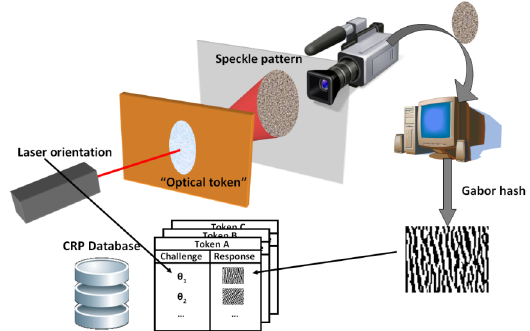
\includegraphics[width=0.8\textwidth]{img/optical-PUF.png}
    \caption{Example of an optical PUF \cite{PUF-study-2010}}
    \label{fig:optical-puf}
\end{figure} 

\subsubsection{Arbiter PUF (A-PUF)}
The idea that delays in integrated circuits (ICs) can be used in PUFs was first introduced by \cite{10.1145/586110.586132}, such PUFs that exploit the delays in ICs are known as Delay-Based PUFs. The specific MUX-chain architecture that defines the Arbiter PUF (A-PUF) as we know it today was later introduced by \cite{9d14141c05ac4f57864d59873ec23799}. The A-PUF is a Delay-Based PUF that exploits the fact that when two electrical signals are launched simultaneously through two identical paths, manufacturing variations will cause one signal to arrive slightly earlier than the other. The A-PUF uses a chain of $n$ multiplexers (MUX) stages, where each stage is controlled by the $n$-th bit of the challenge which determines whether the two signals are crossed over or pass straight through. Due to unavoidable manufacturing differences, the two paths accumulate slightly different delays and an arbiter at the end, typically a D flip-flop, measures which signal arrived first and accordingly produces a response bit of 1 or 0. As seen in figure \ref{fig:A-PUF}, an A-PUF with 128 stages has 128 input bits, which means it has $2^{128}$ possible challenges, as such the A-PUF is considered a strong PUF. However, the additive nature of the delay model that gives the A-PUF its large CRP space also constitutes its primary vulnerability. \cite{10.1145/1866307.1866335} demonstrated that the input-output behavior of the A-PUF can be modeled using logistic regression. For a 64-bit A-PUF, 95\% prediction rate is achieved with as few as 640 CRPs in 0.01 seconds of training time, and 99.9\% accuracy with 18.050 CRPs in under one second of training. This disqualifies the A-PUF for usage in security protocols since it is predictable given enough CRPs.

\begin{figure}[ht!]
    \centering
    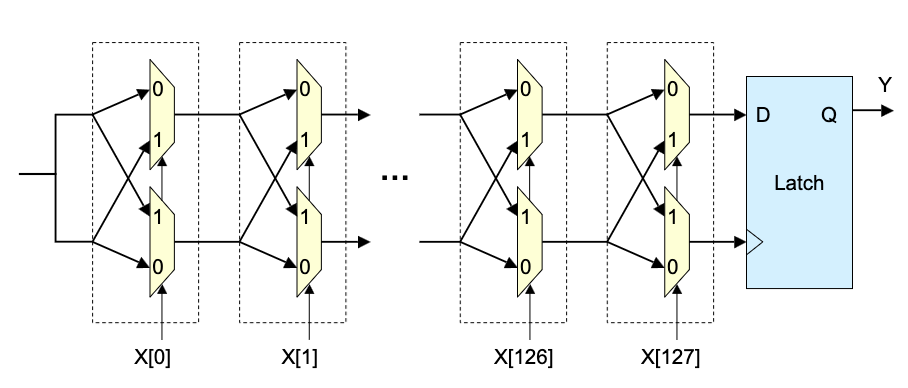
\includegraphics[width=0.8\textwidth]{img/a-PUF.png}
    \caption{Arbiter PUF circuit \cite{10.1145/1278480.1278484}}
    \label{fig:A-PUF}
\end{figure} 

\subsubsection{Ring Oscillator PUF (RO-PUF)}
Initially introduced by \cite{10.1145/1278480.1278484}, the Ring Oscillator PUF (RO-PUF) is a Delay-Based PUF that derives its uniqueness from the differences in oscillation frequencies of multiple identical ring oscillators. Ring oscillators are closed loops of an odd number of inverters whose frequency is determined by the propagation delay of their gates. As seen in figure \ref{fig:RO-PUF}, to generate a sequence of output bits, a fixed sequence of oscillators pairs is selected using the challenge input, and each pair's two frequencies are compared to generate an output bit. Since all the oscillators are identical in design, any frequency difference between them is attributed entirely to manufacturing variations, making the responses unique per device. As mentioned by \cite{10.1145/1278480.1278484}, given $N$ ring oscillators, there are $\frac{N(N/2)}{2}$ distinct pair comparisons. However, the number of truly independent bits is lower than that because the pairwise comparison results are correlated with one another: if oscillator $A$ is faster than $B$, and $B$ is faster than $C$, the outcome of comparing $A$ with $C$ is already implied and contributes no new information. To guarantee fully independent output bits, we can pair each oscillator with exactly one other oscillator, this would yield $N/2$ fully independent response bits for $N$ oscillators, we get fully independent response bits at the cost of requiring more oscillator instances on the PUF. The RO-PUF is therefore considered a weak PUF since its CRP space grows polynomially with the number of oscillators.

\begin{figure}[ht!]
    \centering
    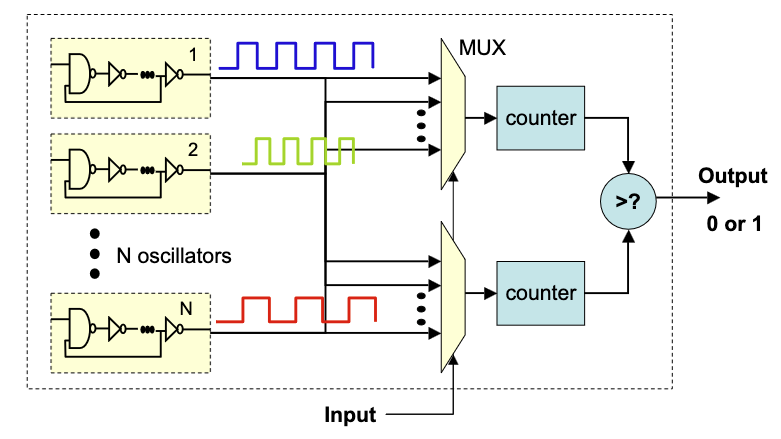
\includegraphics[width=0.8\textwidth]{img/RO-PUF.png}
    \caption{Ring Oscillator PUF circuit \cite{10.1145/1278480.1278484}}
    \label{fig:RO-PUF}
\end{figure} 

\subsubsection{SRAM PUF}
First introduced by \cite{Holcomb2007InitialSS}, the SRAM PUF is a Memory-Based PUF that exploits the random power-up behavior of Static Random Access Memory (SRAM) cells, each of which uses a positive feedback loop to settle into and maintain one of two stable states representing either a 0 or a 1. As seen in figure \ref{fig:SRAM-PUF}, the $V_{th}$ differences in the transistors cause the SRAM cell to start as either 0 (when $A=0, B=1$) or 1 (when $A=1, B=0$) when first powered on. Under normal operations, a write operation forces the cell into one of these states. However, when the SRAM is powered on initially without a preceding write operation, the cell briefly goes into a metastable state in which, theoretically, the feedbacks driving it toward 1 and 0 are perfectly balanced, but in practice, small threshold voltage mismatches between the transistors cause one feedback loop to be slightly stronger than the other, thereby making the cells produce either a 1 or 0. These differences are unavoidable and introduced by the manufacturing process. When the two feedback loops are nearly equal in strength, environmental fluctuations can cause a cell to deviate from its normal state, which results in a bit flip. Error correction is therefore necessary for reliable response generation. The key recognition which allows SRAM PUFs to easily be error corrected is the fact that any cell that is biased towards 0 or 1 will remain strongly biased toward its starting state. Therefore, through repeated measurements, we can assess the stability of each cell and only use the most stable cells for key generation. Although in practice, we also need to use error-correcting codes along with the initial filtering for reliable and reproducible responses. The SRAM PUF is a weak PUF since we get as many output bits as we have cells. The challenge can be which SRAM cell addresses to read or simply the entire SRAM.

\begin{figure}[ht!]
    \centering
    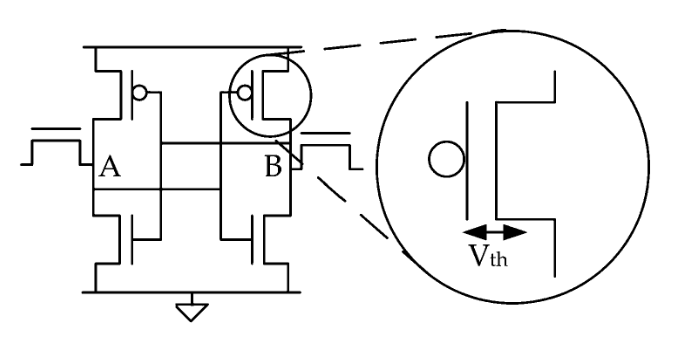
\includegraphics[width=0.8\textwidth]{img/SRAM-PUF.png}
    \caption{SRAM cell \cite{6823677}}
    \label{fig:SRAM-PUF}
\end{figure} 


\subsection{PUF Threats and Attacks}
While PUFs offer interesting security properties by deriving secrets from uncontrollable manufacturing variations, they are not immune to attacks. The security depends heavily on the PUF architecture used and the capabilities of the adversary. Previous research has identified and demonstrated  several classes of attacks that can compromise PUF security. From machine learning attacks that exploit the structure of the PUF's challenge-response behavior to physical side-channel attacks that bypass the CRP interface by monitoring the unintended emissions of the device, many attacks against PUFs are possible. We will now see some of them.

\subsubsection{Machine Learning / Modeling Attacks}
Machine learning (ML) attacks are the most studied and practically demonstrated threat against PUFs and constitute the primary security concern for strong PUF architectures such as the Arbiter PUF. The adversary is assumed to have temporary access to the PUF, during which they collect a large set of challenge-response pairs by querying the PUF. These CRPs are then used to train a mathematical model that can approximate the behavior of the PUF. After training, the model can predict the PUF's response to previously unseen challenges with very high accuracy. \cite{10.1145/1866307.1866335} demonstrated that a 64-bit Arbiter PUF can be modeled using logistic regression with prediction accuracies of more than 99\% with as few as 10,000 CRPs, while more complex architectures such as XOR Arbiter PUFs, which were initially introduced as a countermeasure to protect Arbiter PUFs against ML attacks, were shown to still be vulnerable to modeling attacks using linear regression, although the number of CRPs and training time required for modeling is significantly higher than what is needed for a simple unprotected Arbiter PUF. For example, modeling a 64-bit XOR Arbiter PUF with 6 XORs requires around 200,000 CRPs and takes 31:01 hours. The fundamental reason for this vulnerability lies in the additive delay model behind the Arbiter PUF's behavior since the responses are determined by a linear function of the challenge bits, which can be learned given enough CRPs. 

\subsubsection{Physical Attacks}
Physical attacks involve direct observation of the PUF as a physical object rather than capturing its CRPs. \cite{6581556} were able to physically clone an SRAM PUF using Focused Ion Beam (FIB) circuit edit. While such physical attacks require very expensive machinery and high expertise, they remain realistic for a sufficiently supported and motivated adversary. The mere existence of such successful physical cloning attacks undermines the foundational security assumption on which PUFs are based, which is that the physical characteristics introduced by the manufacturing process are impossible to replicate.

\subsubsection{Side Channel Attacks}

Side-channel attacks are carried out by observing the physical emissions produced by the device during PUF querying. Simple Power Analysis (SPA) is a technique that measures power consumption while executing some algorithm. Since different operations have different power consumption patterns, one can distinguish an addition operation from a multiplication operation simply by looking at the power consumption patterns. If the algorithm handles some secret data like a key bit by bit and runs different operations based on if the bit is a 0 or a 1, then extracting the key from the power consumption chart is obvious. As seen in figure \ref{fig:SPA}, 1 bits appear as tall bumps and 0 bits as short bumps. However in practice, noise prevents such clear distinction between 1s and 0s. Differential Power Analysis (DPA) is typically used rather than SPA to account for the noisy power consumption patterns. DPA is a statistical method for identifying data-dependent correlations from power consumption \cite{AnySiliconDPA}. 

\begin{figure}[ht!]
    \centering
    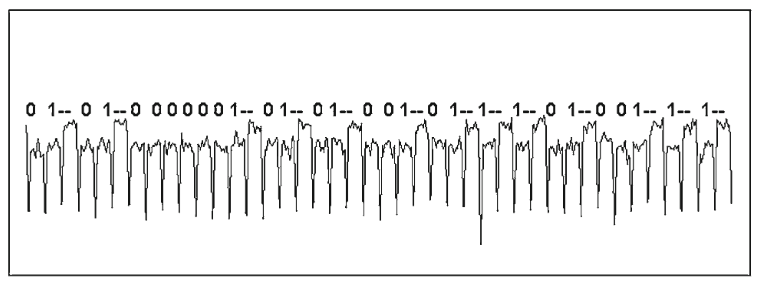
\includegraphics[width=0.8\textwidth]{img/SPA.png}
    \caption{SPA leaks from an RSA implementation \cite{Kocher2011}}
    \label{fig:SPA}
\end{figure} 

The same attacks can also be applied to electromagnetic leakage (EM) since power consumption is proportional to the current demanded by the circuit, and current is just a flow of electrons, and this flow of electrons produces an electromagnetic field which can be measured. One downside of doing power analysis using EM leakage is the fact that the probe must be placed right on top of the area of interest so as not be impacted by the EM radiation from neighboring events (see figure \ref{fig:EM-probe}). Using this principle, \cite{11316252} were able to determine the frequency of one of the ROs involved in one of the challenges of the PUF by measuring EM traces along a grid of points near the FPGA where the RO PUF is implemented. As demonstrated by \cite{10.1007/978-3-642-21599-5_3}, it is also possible to attack the fuzzy extractors, which are used to error-correct the noisy PUF outputs, to extract the generated key.

\begin{figure}[ht!]
    \centering
    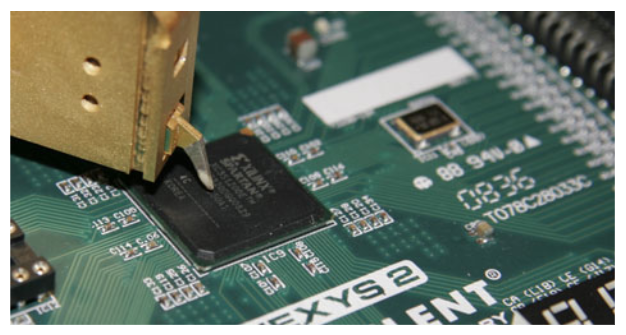
\includegraphics[width=0.5\textwidth]{img/EM-measure.png}
    \caption{EM probe over an FPGA chip \cite{10.1007/978-3-642-21599-5_3}}
    \label{fig:EM-probe}
\end{figure} 


\subsection{Error Correction and Fuzzy Extractors}
Since PUF responses are noisy due to environmental variations, they cannot be used directly as cryptographic keys. Initially introduced by \cite{Dodis_2008}, Fuzzy Extractors are a cryptographic tool for generating a stable secret key from a noisy source such as PUF responses or biometric measurements. A fuzzy extractor consists of two procedures: \textbf{Generate} (Gen) and \textbf{Reproduce} (Rep). As seen in figure \ref{fig:fuzzy}, The Gen function takes a noisy input $w$ and generates a secret key $R$ and public helper data $P$. In a subsequent measurement, we get a noisy input $w'$, the Rep function takes $w'$ and the public helper data $P$ and reproduces the secret key $R$.

The code-offset method shown by \cite{Maes_2016} is an example of how a Fuzzy Extractor can be used to generate a key from a PUF response. As seen in figure \ref{fig:code-offset}, a PUF-based key generator has two phases: Enrollment and reconstruction. The following happens during enrollment:
\begin{enumerate}
    \item A random number generator (RNG) generates a random seed $S$.
    \item A key derivation function (KDF) generates a secret key $K$ using the seed $S$.
    \item The seed $S$ is encoded using an error-correcting code to produce a code word $C$.
    \item The PUF is queried to produce a response $X$.
    \item The response $X$ is XORed with the code word $C$ to produce helper data $W$
    \item The helper data $W$ is stored publicly and the key $K$ is enrolled; enrollment of the key means that we associate its identity with some helper data $W$ and some challenge $C$ that produced the response $X$. After enrollment the key can be discarded since we can reconstruct it in the reconstruction phase.
\end{enumerate}
The reconstruction phase does the following:
\begin{enumerate}
    \item To reconstruct the enrolled key $K$, we first query the PUF to get the noisy response $X'$ using the same previous challenge $C$.
    \item The helper data $W$ associated with the key $K$ is then XORed with the noisy response to produce a noisy code word $C'$.
    \item The noisy code word $C'$ is decoded using the same error correction code used to encode it.
    \item The decoded seed $S'$ is given to the KDF to generate the reconstructed key $K'$.
    \item If the subsequent noisy PUF response $X'$ is close enough to the original response $X$, then the keys $K$ and $K'$ will be identical.
\end{enumerate}

The success of the reconstruction phase depends on whether the noisy PUF response $X'$ is sufficiently close to the original response $X$. If the number of flipped bits exceeds the error correction capability $t$ of the chosen error-correction code, the decoder will produce an incorrect seed $S'$, resulting in a different key $K'$. However, the usage of public helper data is not without flaws. \cite{6965637} demonstrated that attackers could use the public data to infer information about the PUF's response and also manipulate said helper data to recover the secret key by observing system failure rates.


\begin{figure}[ht!]
    \centering
    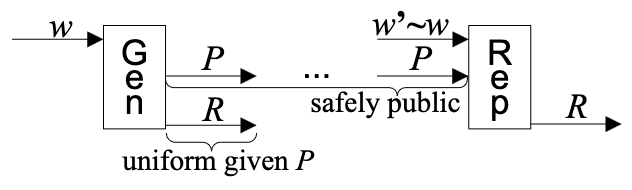
\includegraphics[width=0.8\textwidth]{img/fuzzy-extractor.png}
    \caption{Fuzzy extractor \cite{Dodis_2008}}
    \label{fig:fuzzy}
\end{figure} 


\begin{figure}[ht!]
    \centering
    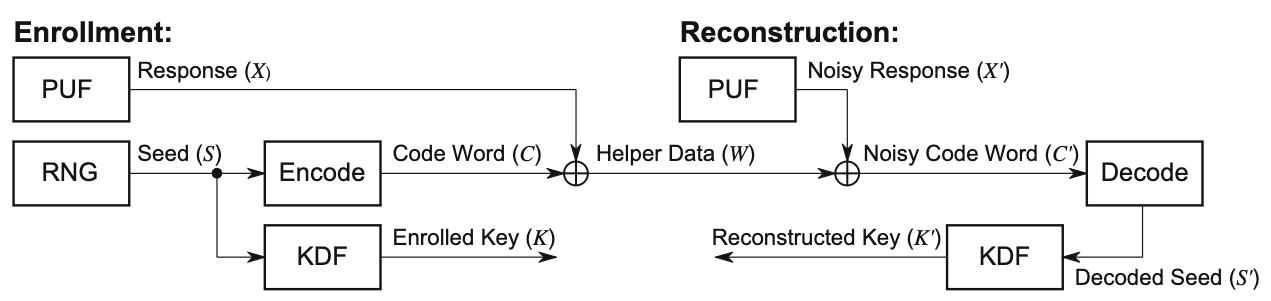
\includegraphics[width=1\textwidth]{img/code-offset.png}
    \caption{PUF-based key generator based on the code-offset method \cite{Maes_2016}}
    \label{fig:code-offset}
\end{figure} 


\subsection{Applications of PUFs}
% Find examples in https://dl.acm.org/doi/epdf/10.1145/3487060
\subsubsection{Device Authentication}
%with CRP DB: https://ieeexplore.ieee.org/abstract/document/7424628
%without CRP DB: https://www.acsu.buffalo.edu/~mblanton/cse708/pufs-without-database.pdf
One of the most researched applications of PUFs is device authentication. For strong PUFs, the most basic form of PUF-based authentication can be achieved using a database of prerecorded CRPs \cite{10.1145/3487060}. As seen in figure \ref{fig:CRP-DB-Auth}, a device / prover $p$ authenticates with a server / verifier $v$. The protocol has two phases, the enrollment phase (Phase 1) and the authentication phase (Phase 2). During the enrollment phase, the device is enrolled into a database by recording some of its CRPs, this step would be carried out by the manufacturer or organization before distributing the devices. At the end of this phase, each device $d_{id}$ will have a set of its CRPs stored in the database $\Gamma_{id} = \{(c_0, r_0), \dots, (c_n, r_n)\}$. In the authentication phase, the verifier $v$ selects some challenge $c'_i$ associated with the device and sends it to the device. Once the device receives the challenge $c'_i$, the PUF is queried to produce the response $r''_i = \Psi_p(c'_i)$, then the device sends the response $r''_i$ to the verifier. If the received response is identical or close enough to the one recorded in the CRP database ($r''_i \simeq r'_i$), then the device is authenticated, otherwise authentication fails. For higher security, CRPs are only used once to prevent replay attacks. While this challenge-response protocol approach is ideal for strong PUFs that have a large CRP space where we can afford only using a CRP once, weak PUFs cannot be used as efficiently and securely with this protocol. 
\begin{figure}[ht!]
    \centering
    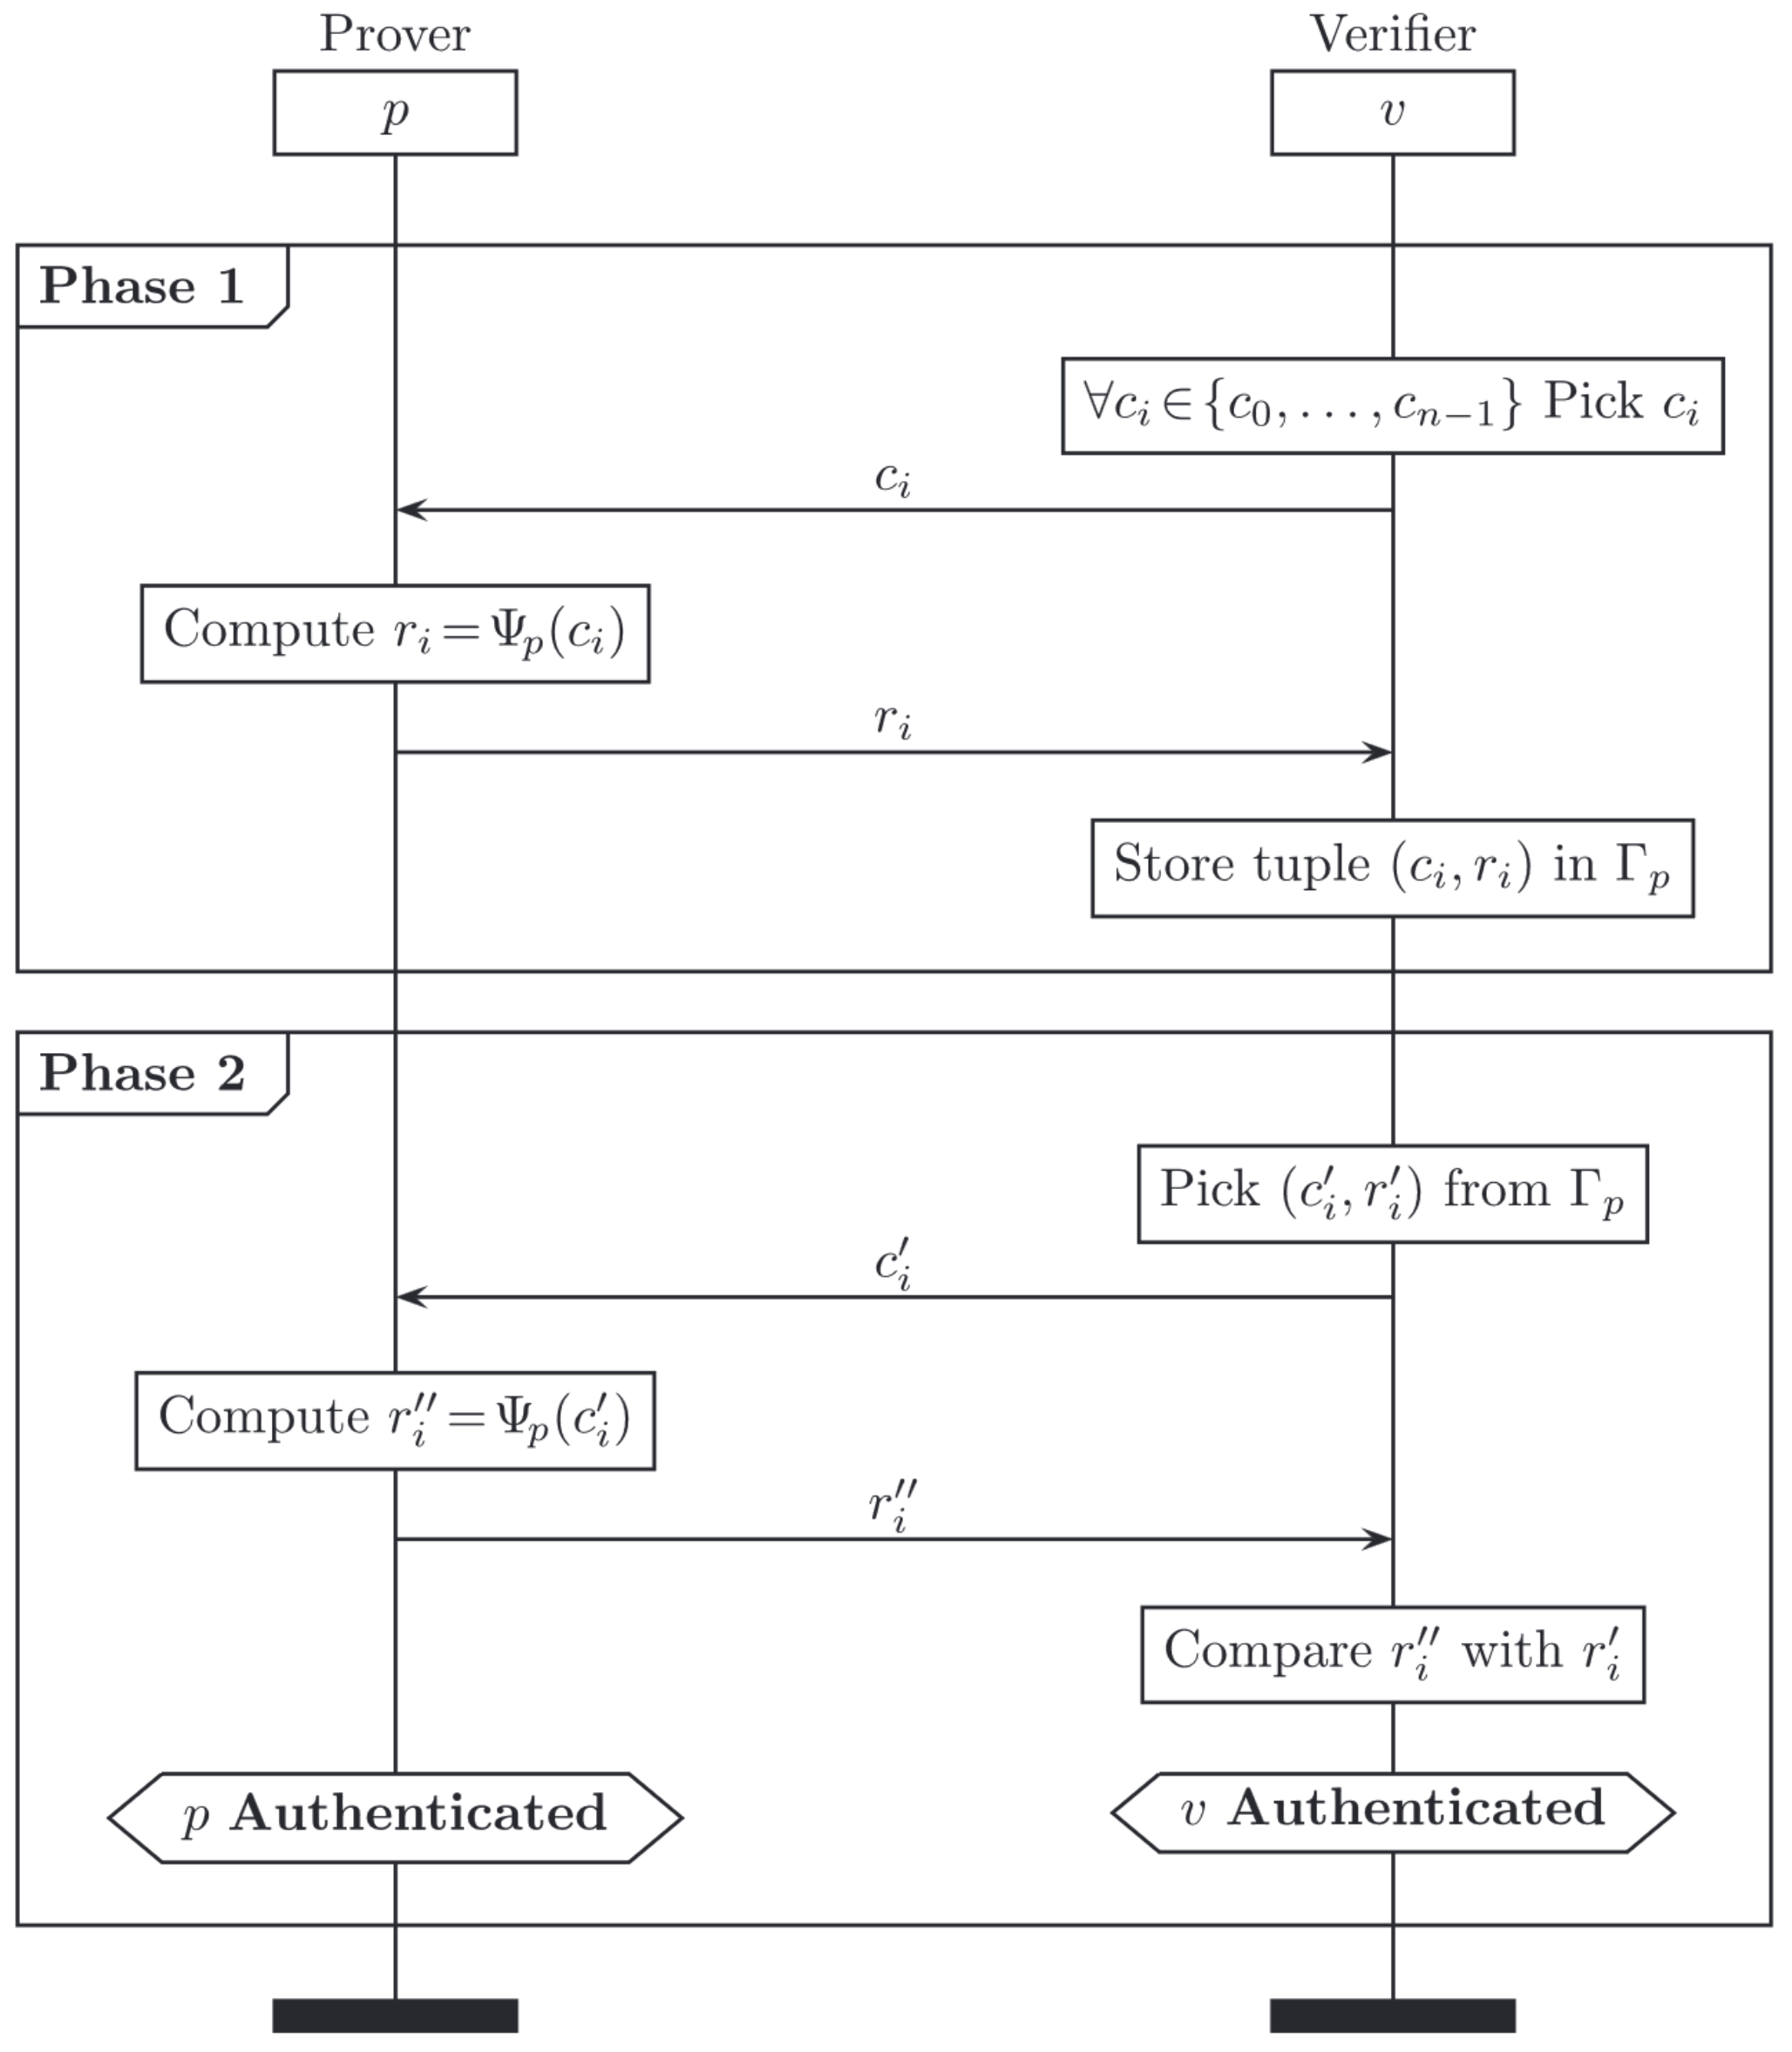
\includegraphics[width=0.7\textwidth]{img/CRP-DB-Auth.png}
    \caption{PUF-based authentication using prerecorded CRPs \cite{10.1145/3487060}}
    \label{fig:CRP-DB-Auth}
\end{figure} 

To achieve authentication, weak PUFs like the SRAM PUF are used as primitives for cryptographic keys or in a similar fashion. As shown by \cite{9233424} on figure \ref{fig:SRAM-Auth}, a fingerprint can be extracted from the SRAM PUF during enrollment and saved, then to authenticate the device, the server sends a nonce and challenge, the device gets the fingerprint from the its SRAM PUF, then to augment the weak PUF, its output $PUF$ is reordered using a challenge to produce $RPUF$, then the response of this authentication request is the hash $H(nonce \space \oplus \space RPUF \space \oplus \space PUF)$, the hash is sent as a response to the server which can in turn verify if the received response matches the expected response. The fingerprint here is a stable construct generated by identifying the most stable bits in the SRAM PUF to only use those that have a stability of 100\%, and an ECC algorithm is used to generate helper data for error correction.
As we can see, when a weak PUF is used in authentication, the device is not required to send its raw PUF responses anymore, but rather the output of the PUF is used to "sign" some nonce to prove to the server that the PUF is there.
\begin{figure}[ht!]
    \centering
    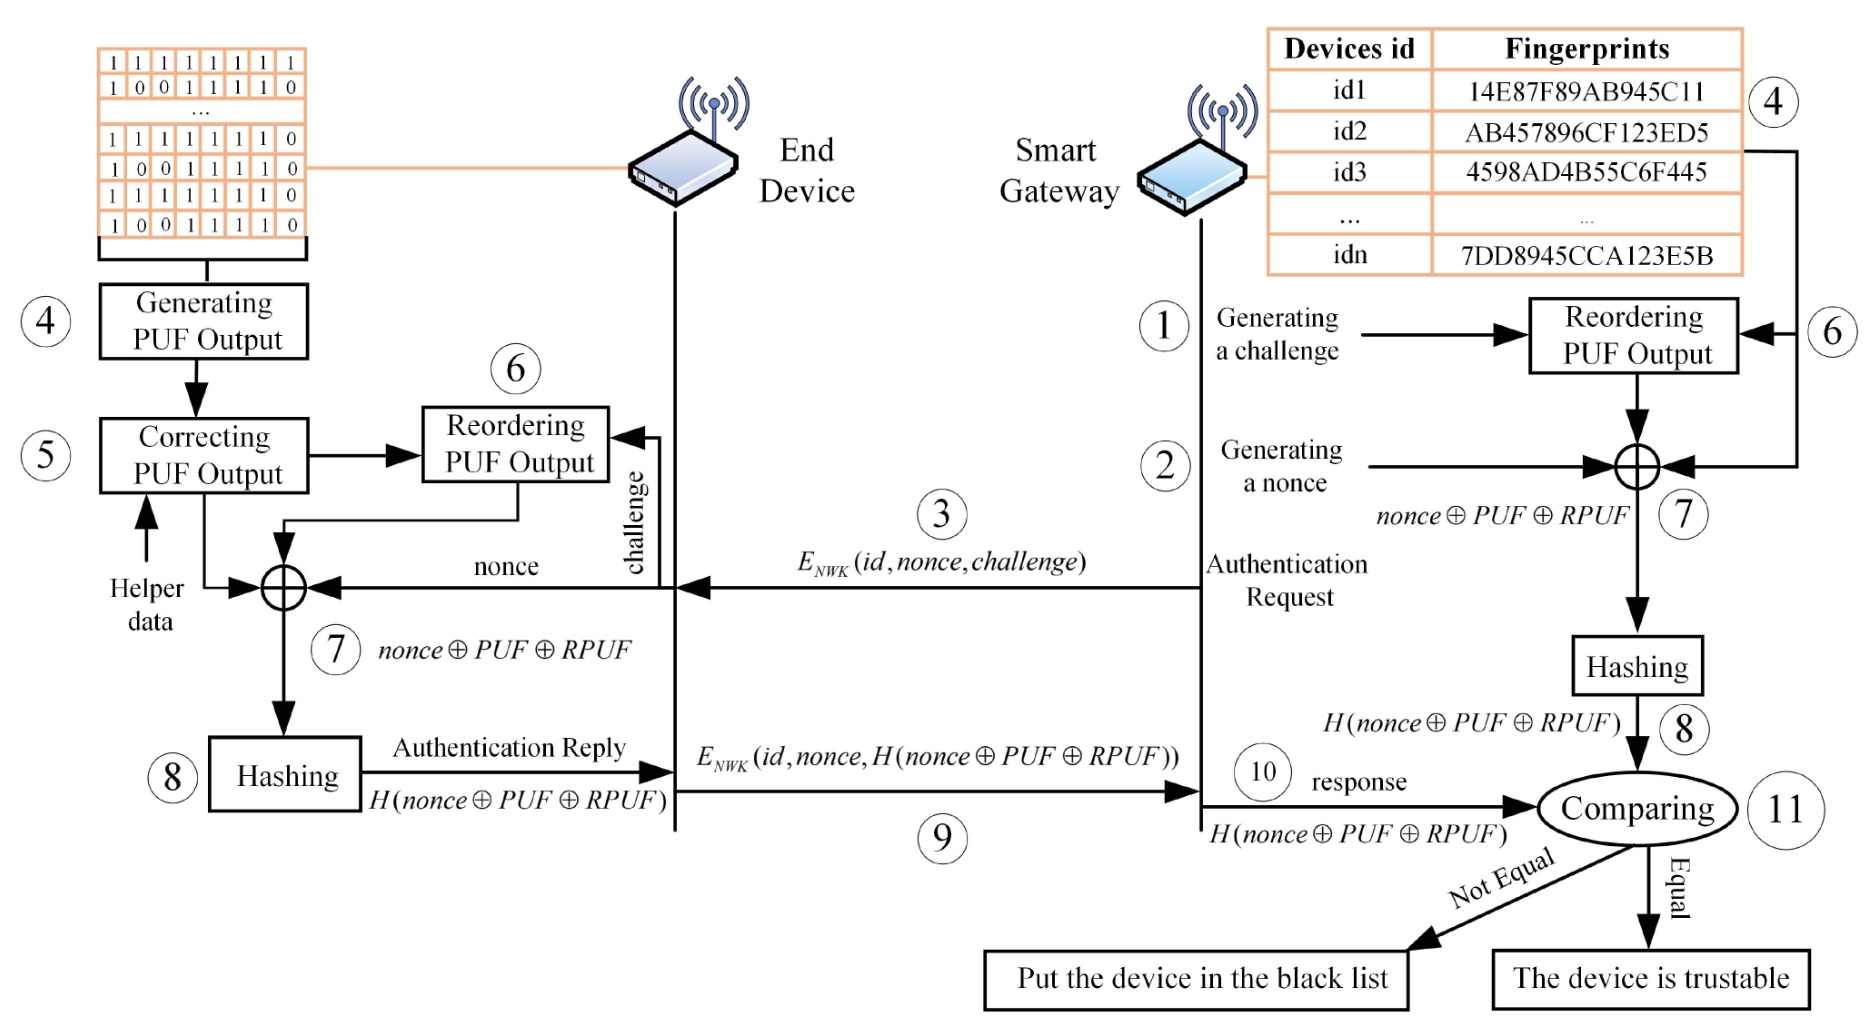
\includegraphics[width=\textwidth]{img/SRAM-Auth.png}
    \caption{Example of PUF-based authentication using a weak PUF \cite{9233424}}
    \label{fig:SRAM-Auth}
\end{figure} 

\subsubsection{IP Protection}
PUFs can be used for hardware intellectual property (HW-IP) protection of FPGA design. The bit-stream used to program the FPGA usually lives on some sort of non-protected flash memory. When the FPGA is powered on, the bit-stream is loaded onto the FPGA to configure it. During this loading phase, an attacker can easily tap into the wires between the flash memory and the FPGA to copy the bit-stream. If this bit-stream is illegally copied, it can lead to revenue loss since using such IP requires licensing. PUFs are used in this context to generate the keys which encrypt this bit-stream when stored in flash memory, then when the FPGA chip receives the encrypted bit-stream, it uses an internal PUF implemented within the FPGA chip to derive a key to decrypt the bit-stream and configure the FPGA, as shown by \cite{4380646}.

\subsubsection{Secure Boot}
Secure boot is a mechanism that ensures a device only executes authorized and unmodified firmware at startup to protect against attacks where the legitimate firmware is replaced with malicious firmware before the device powers on. PUFs can be used as hardware root of trust for a secure boot. As mentioned by \cite{SecureBootPUF2024}, classical secure boot approaches often rely on one public key used by all devices to verify integrity, if its private key is compromised then all devices are compromised. PUFs eliminate this problem entirely by deriving one unique key per device with no key ever getting stored on the device. As such, \cite{SecureBootPUF2024} proposed a PUF-based secure boot mechanism for RISC-V architecture in which the secure element retrieves a boot key from the PUF using a boot challenge stored in one-time programmable memory.

\subsubsection{Random Number Generation}
Beyond key generation and authentication, PUFs can also serve as a source of true random numbers, which are essential for generating nonces, session keys, and initialization vectors. For example, the same random settling of bistable cells at power up that makes SRAM cells useful as a PUF can be exploited as a source of entropy for random number generation. The SRAM cells where the two feedback loops are equal in strength are more susceptible to random noise and therefore settle unpredictably, making them a good source of randomness. \cite{4674345} made this observation and developed the FERNS method (Fingerprint Extraction and Random Numbers in SRAM). At power-up, 0-skewed or 1-skewed cells will power-up to 0 or 1 respectively regardless of the noise conditions in most cases (light cells with low entropy in figure \ref{fig:SRAM-Rand}), such cells will form the basis of the fingerprinting to provide identification. Whereas neutral-skewed cells, that do not have a strong tendency toward either state can powerup to either 0 or 1 (dark cells with high entropy in figure \ref{fig:SRAM-Rand}), will provide randomness, making the SRAM serve as both a PUF and a TRNG. As such, they demonstrated that a 512-byte SRAM fingerprint contains sufficient entropy to generate 128-bit true random numbers and that the generated numbers pass the NIST randomness tests. One limitation of this approach is that the entropy is only generated during power-up, which is less practical than a dedicated TRNG circuit that can be queried at any time, but it comes with the advantage that no extra circuit is needed.

\begin{figure}[ht!]
    \centering
    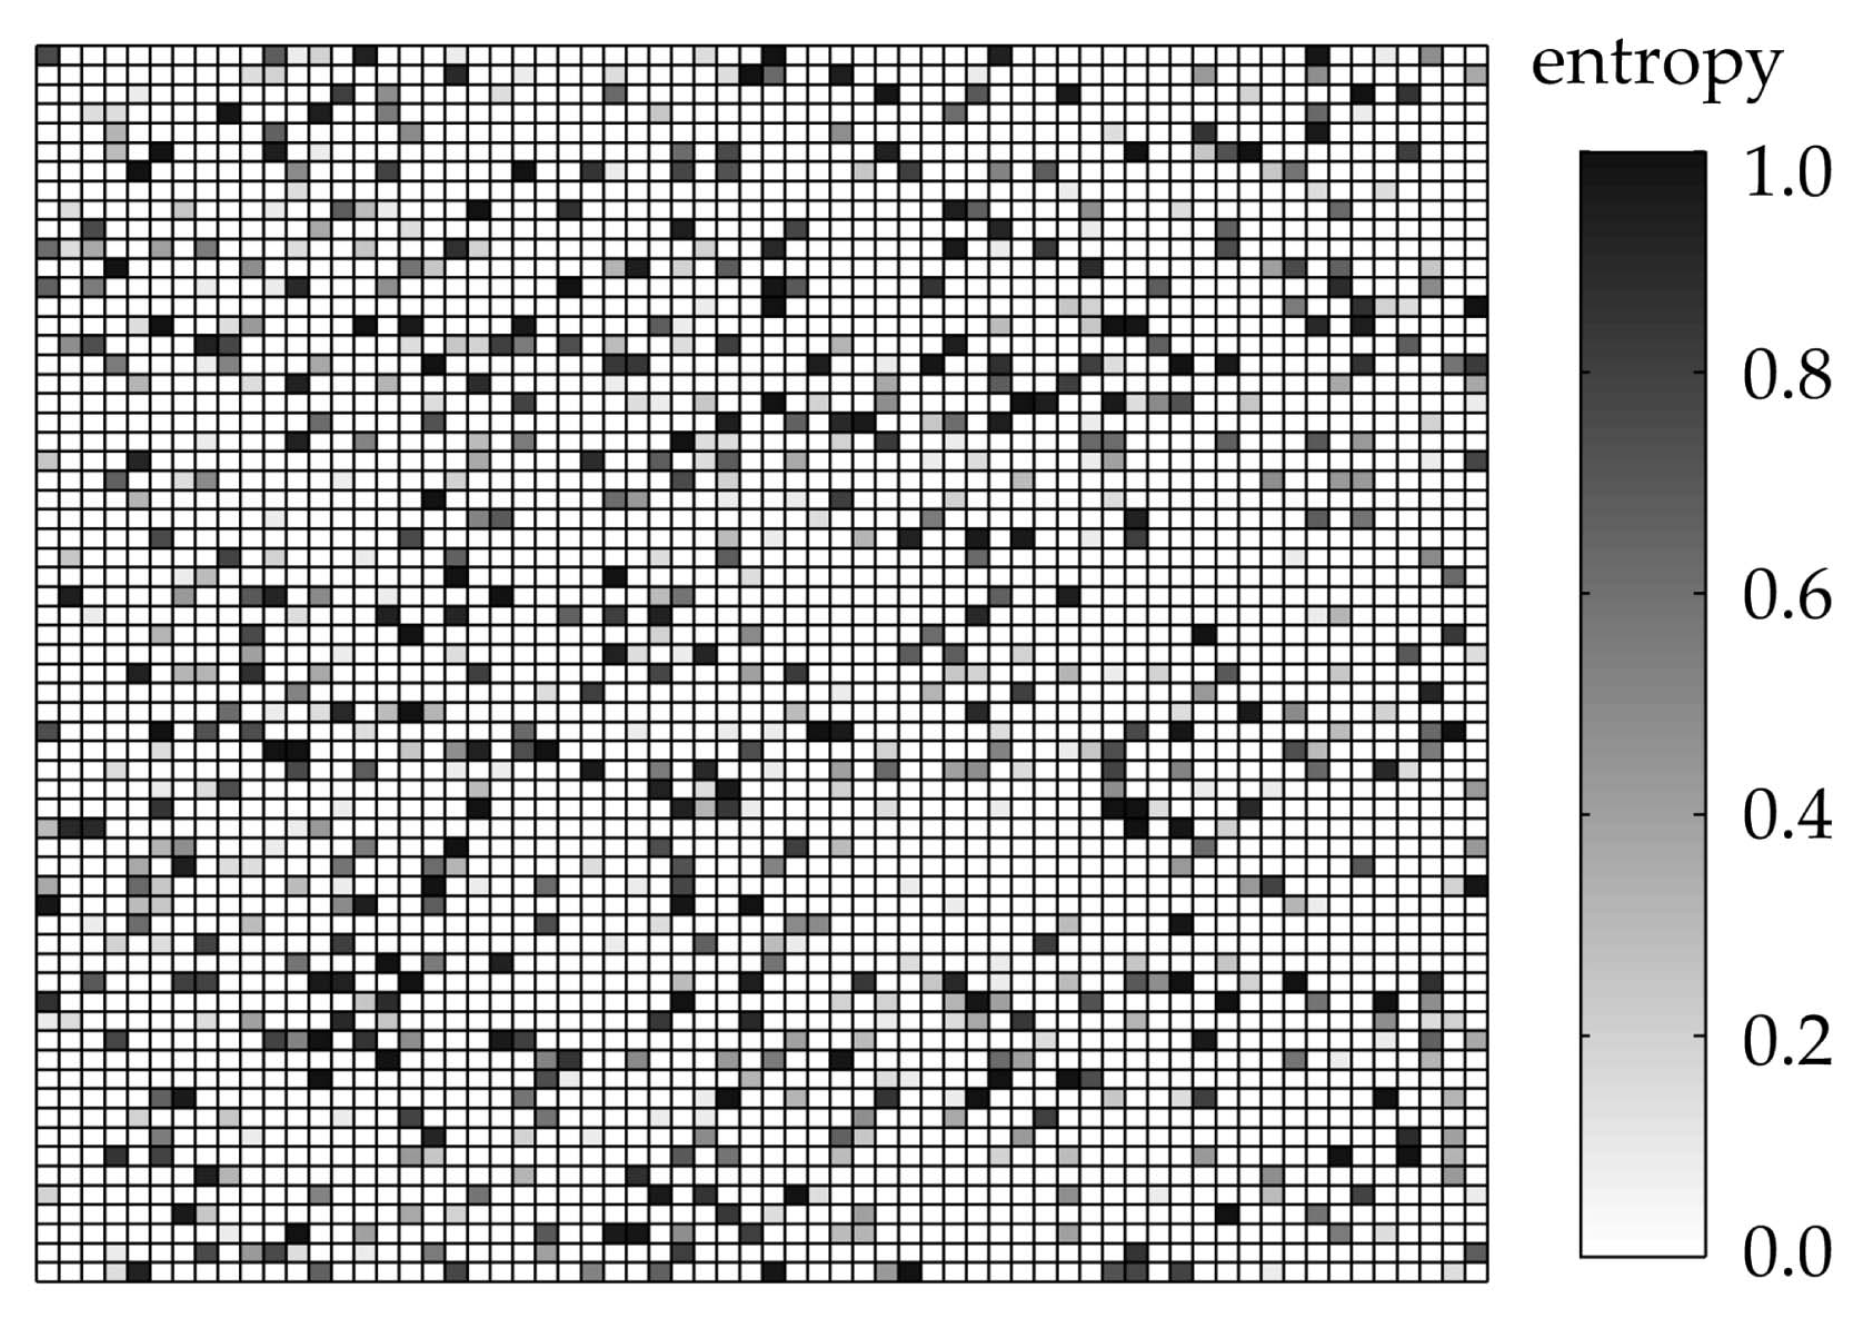
\includegraphics[width=0.8\textwidth]{img/SRAM-Rand.png}
    \caption{SRAM cells entropy determined from 100 power-ups at 294 K. \cite{4674345}}
    \label{fig:SRAM-Rand}
\end{figure} 

\section{CHOICE PUF}

The CHOICE PUF introduced by \cite{9556423} is a delay-based weak PUF or more accurately a delay-tunable PUF. Indeed, its main novelty is the fact that it is tunable, meaning that by changing the challenges a certain way, it is possible to increase or decrease the probability of obtaining 1s in the PUF response. This tuning property also allows us to find at least one challenge per FPGA board type that has the lowest bit-error rate (BER) and ideal uniqueness and uniformity. Although the authors claim that the CHOICE PUF has a low footprint on the FPGA, our testing of their implementation on other boards showed that the CHOICE PUF takes a considerable amount of FPGA slices since each PUF cell needs four 32-bit addressable shift registers (ASRs). In this section, we will explain the inner workings of the CHOICE PUF. This PUF architecture warrants its own section because it is the PUF we used for the REPUSH protocol implementation.

\subsection{Addressable Shift Register (ASR)}
To understand the CHOICE PUF architecture, we must first understand how ASRs operate. ASRs are sequential logic circuits that can be used to store serial data. As seen in figure \ref{fig:ASR}, an ASR is a chain of D flip-flops with a multiplexer at the end. A D flip-flop (D-FF) captures the value present at its data input \verb|D| on an active clock signal (\verb|CE=1| and rising \verb|clk| edge) and holds that captured value as its output \verb|Q| until the next active clock signal which can change its content again based on what the data input is, thereby acting as a single-bit memory. In the ASR, $S$ number of such flip-flops ($q_0, q_1, \dots,q_{S-1}$) are connected in series such that the output of each stage feeds the data input of the next, and on each active clock edge (gated by signal \verb|ce|), the input signal \verb|d| is captured into the flip-flop $q_0$ while every subsequent flip-flop captures the value of its predecessor, propagating the data one stage forward through the chain. The ASR exposes the output of each of its flip-flops through a multiplexer (MUX) which accepts as input an address $a$ as a bus of length $\log_2(S)$, the address $a$ is an integer in binary format which determines which flip-flop's output to read out into the MUX's output \verb|Q|. A selected flip-flop $q_i$ will propagate to the MUX with some delay $\tau_i$ since the wires leading from the flip-flops to the MUX are of variable lengths, as we will see later, the CHOICE PUF exploits this fact as part of its delay model. 
\begin{figure}[ht!]
    \centering
    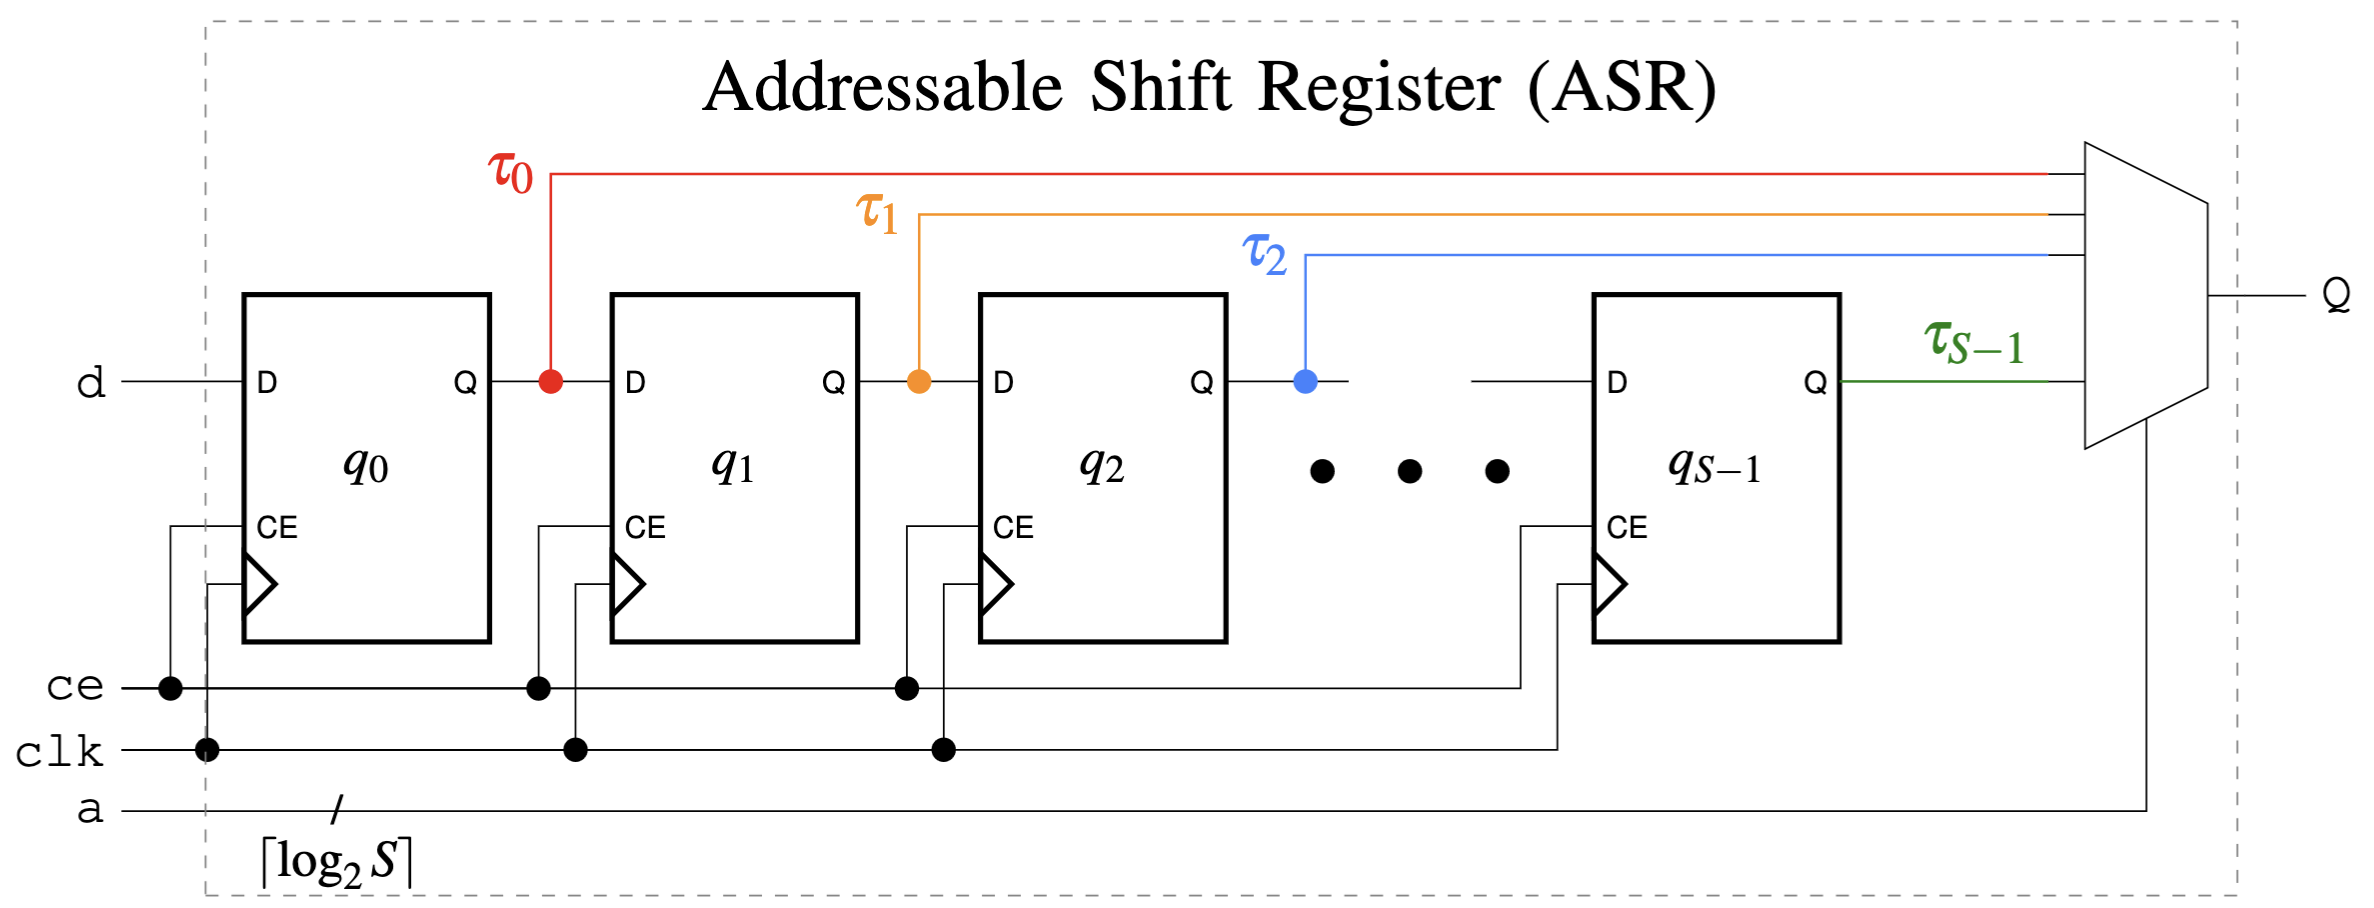
\includegraphics[width=\textwidth]{img/ASR.png}
    \caption{S-stage Addressable Shift Register (ASR). \cite{9556423}}
    \label{fig:ASR}
\end{figure} 
\subsection{PUF Architecture}
As seen in figure \ref{fig:CHOICE-PUF}, a CHOICE PUF cell consists of four 32-bit ASRs ($ASR_0, \dots, ASR_3$) where each ASR controls one corresponding MUX ($MUX_0,\dots,MUX_3$). The output of $o_{MUX_0}$ of multiplexer $MUX_0$ controls the asynchronous set input \verb|PRE| of a flip-flop which will store the PUF output bit, the \verb|PRE| input essentially just makes the flip-flop store something independent of the clock cycle. Each $ASR_i$ can be adjusted via its address input $a_i$ to influence the ASR's propagation delay $\tau_{ASR_i}$, since as we have seen before, inside the ASR, the wires leading to the final multiplexer are of different lengths and thus of different delays. The propagation delay $\tau_{ASR_i}$ is the delay between a change of the output of the ASR's selected internal flip-flop that is selected by address $a_i$ and the occurrence of the signal at the $MUX_i$. Each $MUX_i$ has a logic 0 signal at its 0 position and the output $o_{MUX_{i+1}}$ as its 1 position, except $MUX_3$ which always has a logic 1 signal at its 1 position.    

\begin{figure}[ht!]
    \centering
    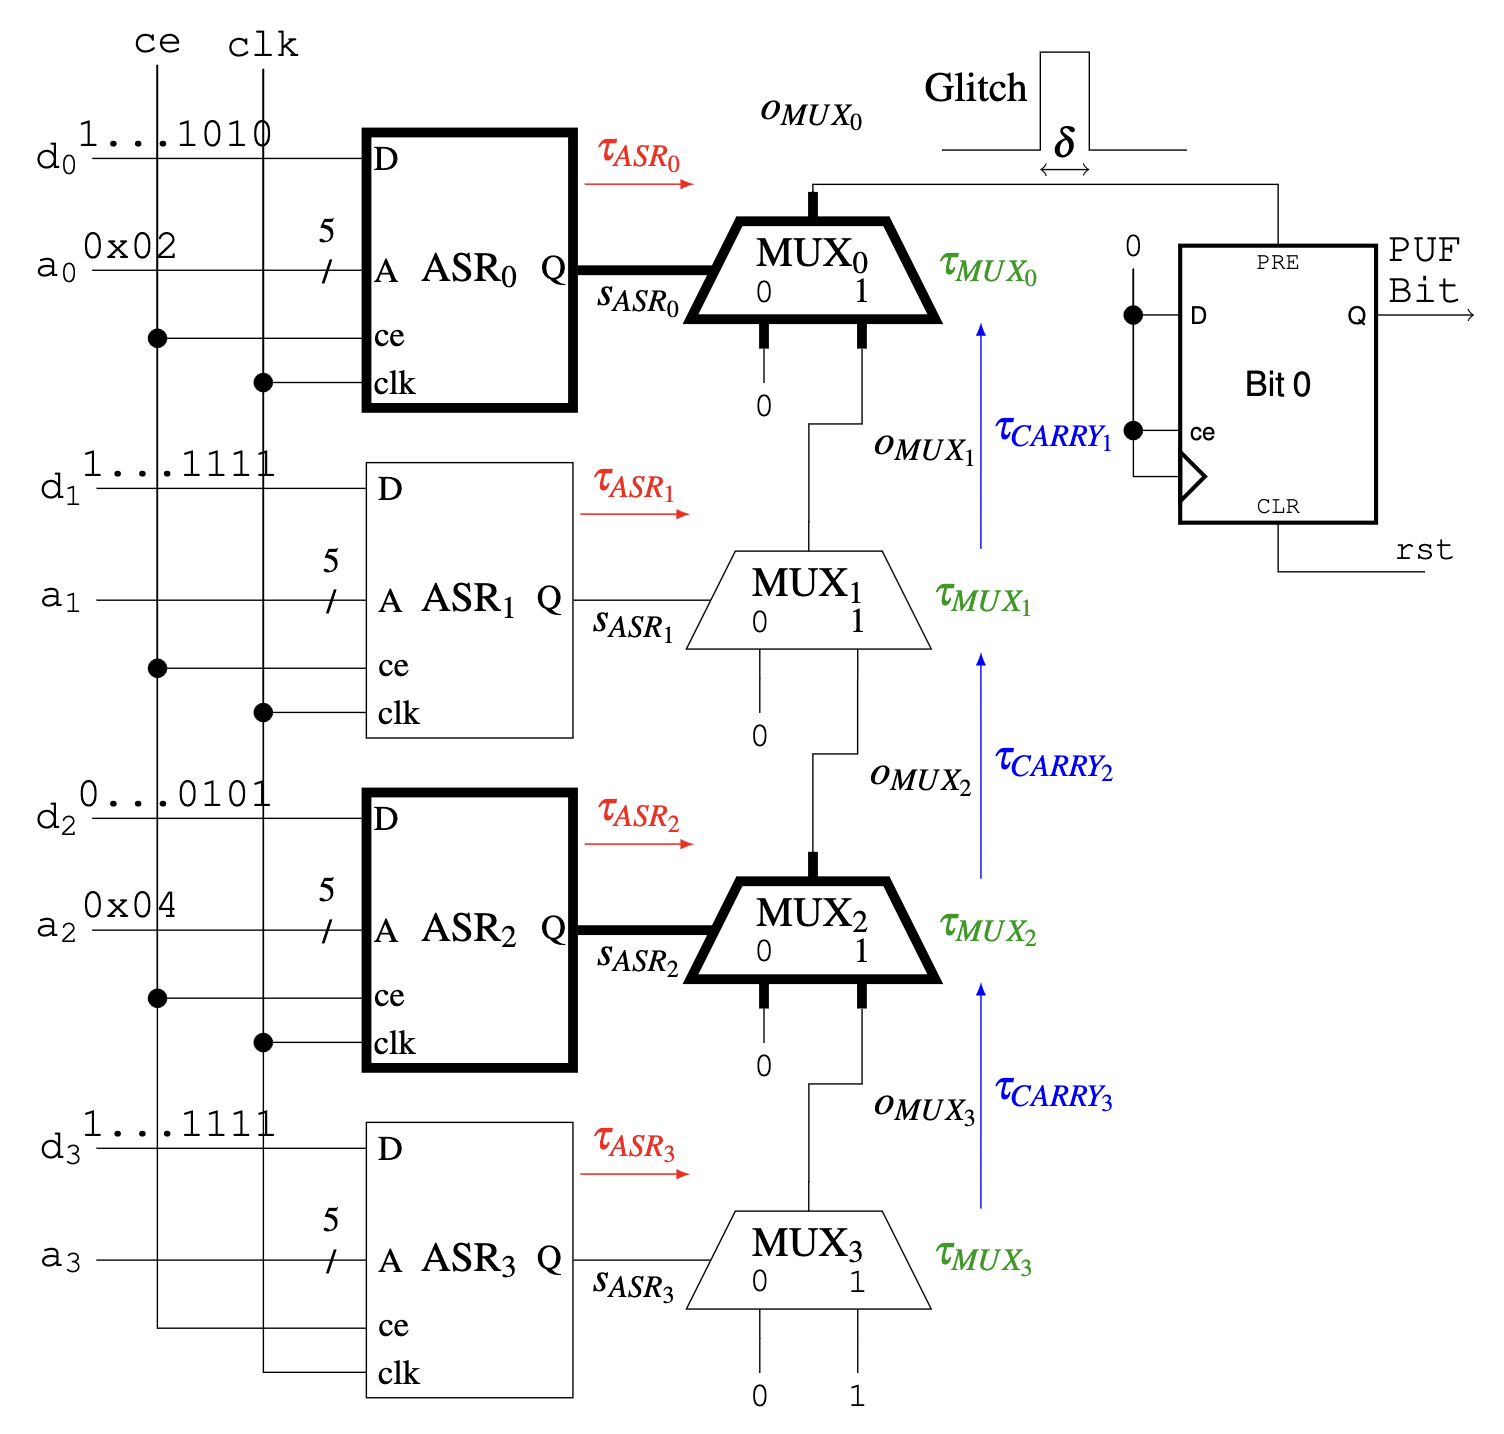
\includegraphics[width=\textwidth]{img/CHOICE-PUF.png}
    \caption{CHOICE PUF cell circuit. \cite{9556423}}
    \label{fig:CHOICE-PUF}
\end{figure}

As part of the PUF challenge, only two of the four ASRs are selected for generating a glitch at $o_{MUX_0}$ (ASRs with a bold outline in the figure \ref{fig:CHOICE-PUF}). The first active ASR will be referred to as $ASR_i$ and the second as $ASR_j$ where $i < j$ and $i,j\in\{0,1,2,3\}$. The two remaining ASRs are considered as inactive since clock cycles will not toggle any signal change on their outputs because they are initialized as all 1s. It is possible to select $\binom{4}{2}=6$ pairs of ASRs as active as part of the PUF challenge. The chosen addresses $a_i$ and $a_j$ of the respective selected ASRs $ASR_i$ and $ASR_j$ are also part of the PUF challenge. As such, we get a total of $\binom{4}{2}\cdot32^2 = 6144$ possible PUF challenges. Each challenge can be defined as a tuple $C=(i,j,a_i,a_j)$. To cause a glitch (small burst of a logic 1 signal) at $o_{MUX_0}$, each ASR must be set with a specific bit pattern $P(k)$ depending on its position $k$ in the PUF cell, as shown in equation \ref{eq:Pk}. Inactive ASRs ($k \notin \{i,j\}$) are initialized with a sequence of all 1s, while $ASR_i$ is initialized either with $1\dots1010$ if $a_i$ is an even address or $0\dots1010$ if $a_i$ is odd. In contrast, $ASR_j$ is initialized with $0\dots0101$ if $a_j$ is even or $1\dots1010$ if $a_j$ is odd.
\begin{equation}
P(k) =
\begin{cases}
1\dots1111 & \text{if } \space k \notin \{i,j\} \\
1\dots1010  & \text{else if } \space k = i \space \land \space a_k\bmod2 = 0 \\
1\dots1010  & \text{else if } \space k = j \space \land \space a_k\bmod2 \neq 0 \\
0\dots0101 & \text{else}
\end{cases}
\label{eq:Pk}
\end{equation}

To get $N$ PUF bits as output, we simply instantiate $N$ PUF cells where we apply the same challenge tuple $C=(i,j,a_i,a_j)$.
\subsection{Querying}
The CHOICE PUF is queried in the following phases:
\begin{enumerate}
    \item Fill (31 cycles): all ASRs are driven bit by bit to fill them with their respective bit patterns $P(k) = d_k$. For the two active ASRs, only the last 31 bits ($d_k[1\ldots31]$) of the bit pattern are initially loaded. The two addresses $a_i$ and $a_j$ are also set during this phase.
    \item Reset: For each PUF cell, the output flip-flop is cleared.
    \item Measurement (1 cycle): For the two active ASRs, \verb|ce| is activated and the first bit $d_i[0]$ of the pattern is driven into the ASRs at the same time to trigger the race.
    \item Settling (2 cycle): We wait for the race to resolve.
    \item Readout: The output flip-flop's bit is captured as the PUF cell's response. 
\end{enumerate}

\subsection{Delay Model}
Whether a PUF cell outputs a 1 or 0 at the end depends on the width $\delta$ of the glitch at $o_{MUX_0}$. The output flip-flop has a minimal glitch width $\delta_{min}$ that is required to successfully drive the \verb|PRE| input and set it to 1 as seen in equation \ref{eq:puf-out-delta}. This minimal glitch width $\delta_{min}$ depends on the resistive and capacitive load (RC) of the routing path from $o_{MUX_0}$ to the output flip-flop since the path acts as a low-pass filter which will ignore glitches that are not wide enough. 

\begin{equation}
PUF =
\begin{cases}
1 & \delta \ge \delta_{min} \\
0 & \delta < \delta_{min} 
\end{cases}
\label{eq:puf-out-delta}
\end{equation}

We shall now derive a formula for the glitch width $\delta$ based on the delays of the PUF cell. For the two selected ASRs, let us consider the delays $\tau_i=\tau_{ASR_i} + \tau_{MUX_i}$ and $\tau_j=\tau_{ASR_j} + \tau_{MUX_j}$, where $\tau_{ASR_k}$ is a delay determined by the chosen address $a_k$ of the ASR and $\tau_{MUX_k}$ is the delay introduced by the routing inside the multiplexer. We also consider $\tau_{CARRY_k}$ as the time required to forward a signal from the output $o_{MUX_k}$ of a multiplexer to the 1-data input of the $MUX_{k-1}$ above it on the carry chain. The delay between the output of $MUX_j$ and the output of $MUX_i$ can be written as:
\[ \tau_{i,j} = \sum_{k=i}^{j-1}\tau_{CARRY_{k+1}}+\tau_{MUX_k} \]
With these definitions of $\tau_i$, $\tau_j$ and $\tau_{i,j}$, there exists three different delay scenarios that would determine the glitch width $\delta$, as seen in figure \ref{fig:CHOICE-PUF-Delay}.
\begin{figure}[ht!]
    \centering
    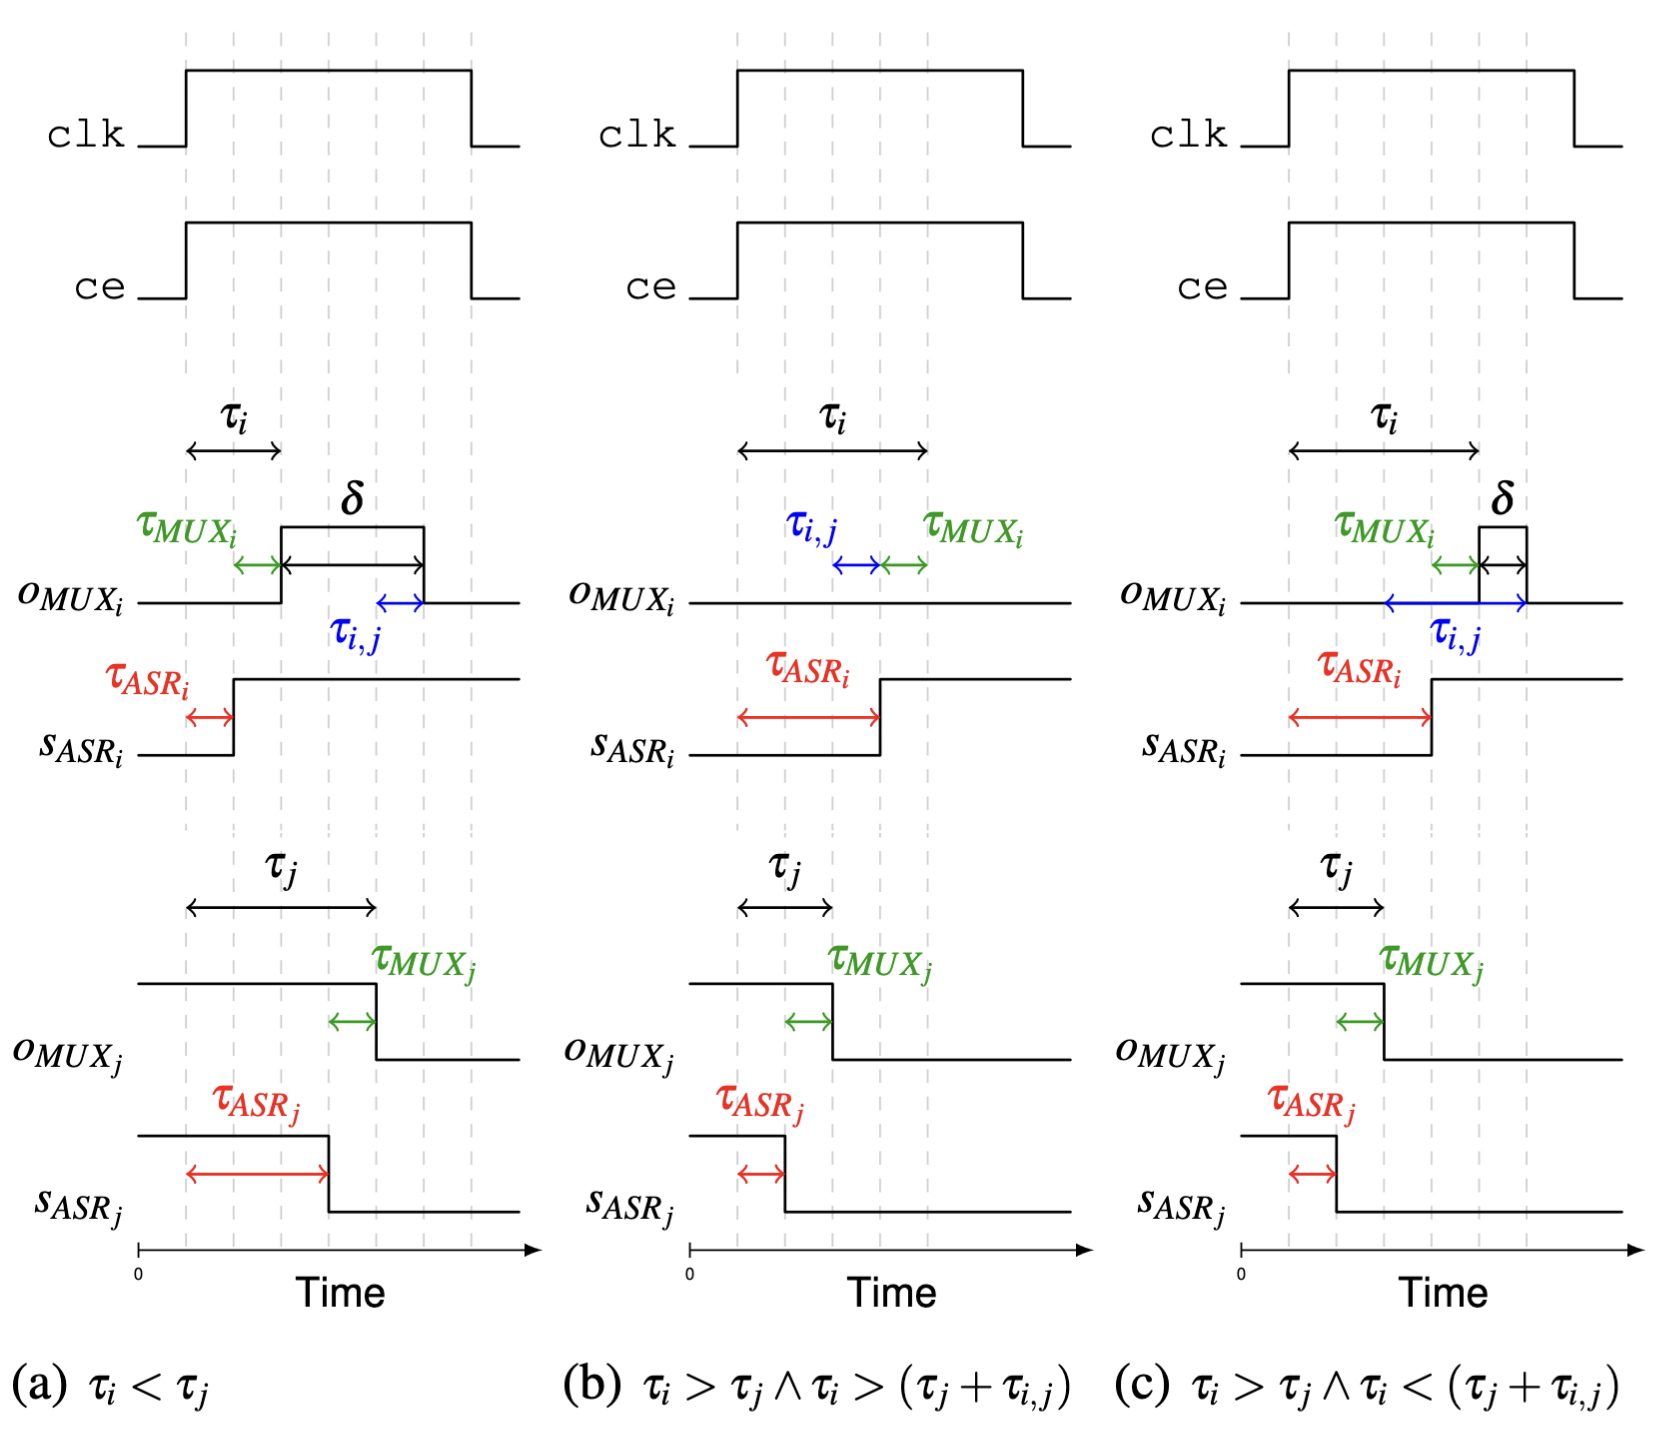
\includegraphics[width=0.8\textwidth]{img/CPUF-Delay-Model.png}
    \caption{CHOICE PUF's three possible delay scenarios. \cite{9556423}}
    \label{fig:CHOICE-PUF-Delay}
\end{figure}

The first case (a) denotes when in the measurement phase the switching of the output signal $s_{ASR_i}$ occurs faster than the switching of the output signal $s_{ASR_j}$, $MUX_i$ propagates the 1 signal from $o_{MUX_j}$ to its output $o_{MUX_i}$ until $MUX_j$ switches to 0, and this is what forms the glitch width $\delta$. Since the delay here is influenced by both the ASR and the multiplexer, we can simplify this case as $\tau_i < \tau_j$, and $\tau_{i,j}$ will contribute greatly to the width of the glitch $\delta$.

When $\tau_i > \tau_j$, $\tau_{i,j}$ becomes decisive in determining whether a glitch will appear at all. As is seen in case (b) where the value of $\tau_{i,j}$ is so small that the output of $o_{MUX_j}$ is always triggered earlier than that of $MUX_i$ and no glitch occurs since $o_{MUX_i}$ stays as 0, this happens if $\tau_{i} > (\tau_j + \tau_{i,j})$.

In the third case (c), $\tau_i$ is still larger than $\tau_j$, similarly to case (b), but this time $\tau_i < (\tau_j + \tau_{i,j})$, i.e. the delay $\tau_{i,j}$ is large enough that $o_{MUX_i}$'s switch to 1 (triggered by $s_{ASR_i}$ after $\tau_i$) still falls inside the window during which the 1 signal coming from $o_{MUX_j}$ is present at the 1-input of $MUX_i$. The observed glitch width is however narrower in this case.

As seen in figure \ref{fig:CHOICE-PUF-Delay}, the created glitch width $\delta$ depends on the absolute differences between $\tau_j+\tau_{i,j}$ and the delay $\tau_i$. It follows that we can estimate $\delta = (\tau_j+\tau_{i,j}) - \tau_i$, and as such we get the equation for the PUF output as:

\begin{equation}
PUF =
\begin{cases}
1 & (\tau_j+\tau_{i,j}) - \tau_i \ge \delta_{min} \\
0 & (\tau_j+\tau_{i,j}) - \tau_i < \delta_{min} 
\end{cases}
\label{eq:puf-out}
\end{equation}

From this we can see that the wider the glitch $\delta$ the higher the probability that we get a 1 as output for the PUF cell, and since this glitch width is dependent on the chosen addresses $a_i$ and $a_j$, then it is possible to find which challenges have the ideal uniformity of 50\%, and this is why the CHOICE PUF is said to be tunable.  


\subsection{Evaluation}
The CHOICE PUF was evaluated on $N=6$ Xilinx Zynq xc7z010clg400-1 boards (labeled $B_0,\dots,B_5$). A 128-bit CHOICE PUF ($Z=128$) was instantiated on each board since 128 bits is a typical length for keys such as an AES key. For every one of the $6144$ possible configurations or challenges $c$ and every board $b$, the PUF was queried $M=1000$ times, yielding responses $r^m_{b,c} \in \{0,1\}^Z$ for $m \in [0,M-1]$. The most frequently occurring response over these $M$ measurements is taken as the nominal response $r^*_{b,c}$, which serves as the reference against which uniformity, uniqueness and reliability are measured.
\begin{figure}
    \centering
    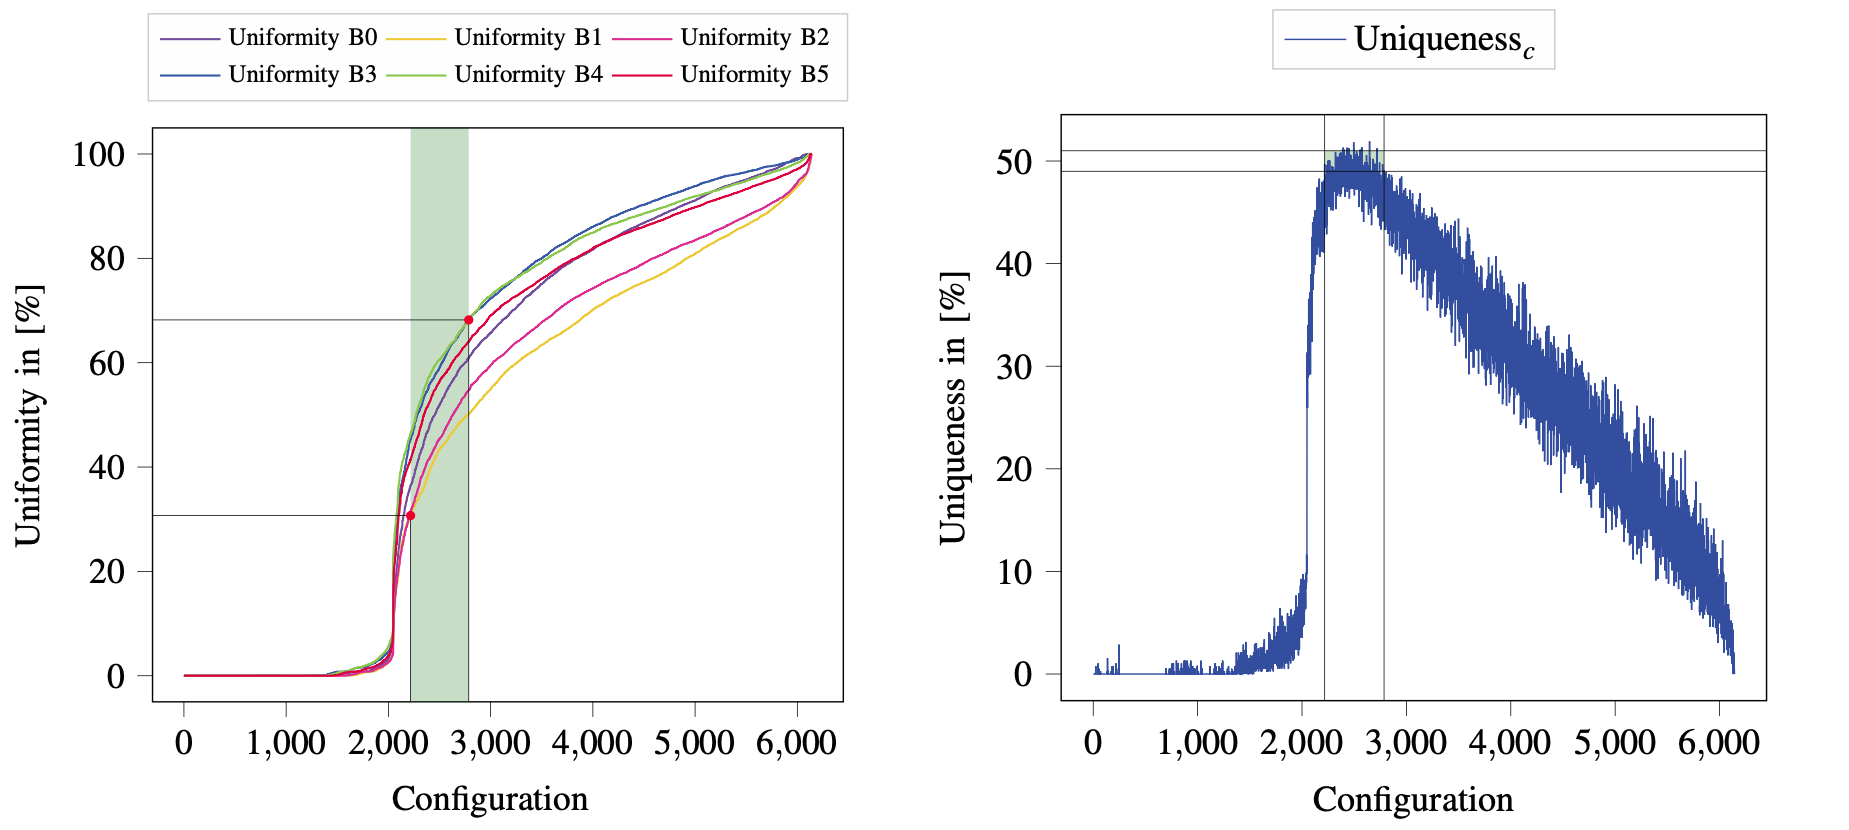
\includegraphics[width=1\linewidth]{img/CPUF-Paper-Unif-Uniq.png}
    \caption{CHOICE PUF uniformity and uniqueness \cite{9556423}}
    \label{fig:CPUF-Paper-Unif-Uniq}
\end{figure}
\subsubsection{Uniformity}
Uniformity measures the proportion of ones in the nominal response:
\begin{equation}
Uniformity_{b,c} = \frac{1}{Z}\sum_{i=0}^{Z-1} r^*_{b,c}(i) \cdot 100\%
\end{equation}
where $r^*_{b,c}(i)$ is the $i$-th bit of the nominal response of board $b$ under configuration $c$. A uniformity close to 50\% is an ideal balance of 0s and 1s in the response, which is desirable for randomness. The left plot on figure \ref{fig:CPUF-Paper-Unif-Uniq} shows the sorted uniformity of all $6144$ configurations for each of the six boards. The curves span the whole range from 0\% to 100\% on every board, which confirms the tunability of the PUF by choosing the appropriate configuration to reach any target uniformity. 

\subsubsection{Uniqueness}
Uniqueness is measured as the average pairwise inter-chip Hamming distance of the nominal responses across all board pairs for a fixed configuration $c$:
\begin{equation}
Uniqueness_c = \frac{2}{N(N-1)}\sum_{i=0}^{N-2}\sum_{j=i+1}^{N-1}\frac{HD(r^*_{i,c},r^*_{j,c})}{Z}\cdot100\%
\end{equation}
A uniqueness close to 50\% is desirable since it means that on average half of the response bits differ between any two boards for the same configuration, which is what allows distinct devices to be differentiated by their PUF responses.
The right plot on figure \ref{fig:CPUF-Paper-Unif-Uniq} shows that uniqueness peaks at around 50\% for the same band of configurations that have uniformity between 30\% and 70\%. Within this band, there are 147 configurations that achieve a uniqueness between 49\% and 51\%, making them the ideal configurations to use in practice.

\subsubsection{Reliability}
Reliability is measured using the Bit Error Rate (BER), which is computed per board and configuration as the average Hamming distance between each of the $M$ measured responses and the nominal response:
\begin{equation}
BER_{b,c} = \frac{1}{M}\sum_{m=0}^{M-1}\frac{HD(r^*_{b,c}, r^m_{b,c})}{Z}\cdot100\%
\end{equation}

An ideal BER of 0\% would mean the PUF's response never changes between measurements, as such, more robust responses tend to have lower entropy. As seen in figure \ref{fig:CHOICE-ber}, on the 147 ideal configuration identified before, the average BER ranges between 2.2\% and 3.8\%, with 13 configurations providing an average BER less than or equal to 2.5\%. To further optimize, each board could select its own best-performing configuration in terms of uniformity and reliability among the 147 to identify itself with.

\begin{figure}
    \centering
    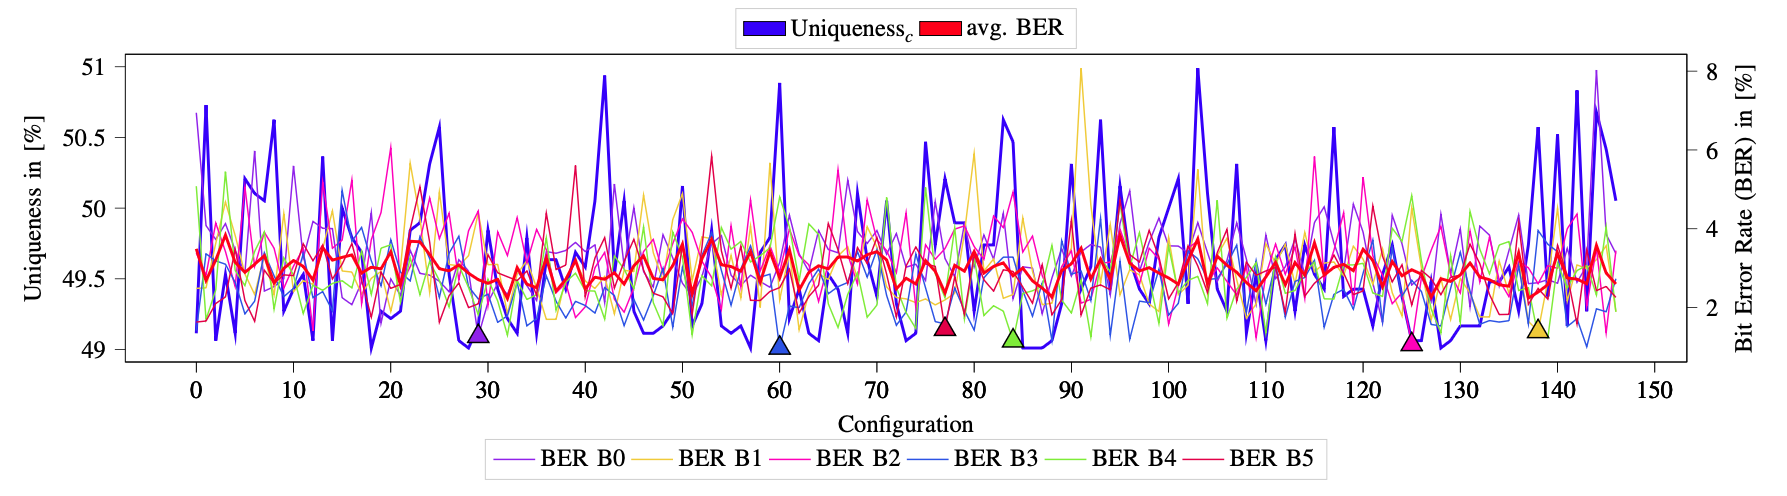
\includegraphics[width=1\linewidth]{img/CPU-BER-Paper.png}
    \caption{Uniqueness and average BER of the 147 ideal configurations \cite{9556423}}
    \label{fig:CHOICE-ber}
\end{figure}

\subsubsection{Footprint}
In the paper, it is mentioned that the CHOICE PUF's footprint is small. However, this is only the case because of the Xilinx SLICEM slice. As we will see in the implementation chapter, the footprint of the CHOICE PUF is quite large when using other FPGA brands.



\section{Logically Reconfigurable PUF (LR-PUF)}
As has been seen in the previous section about PUFs, PUF architectures typically have a fixed challenge-response behavior, this is desirable for applications like device authentication and secure boot since we want the CRP behavior of the device to permanently be tied to its identity. However, other applications would benefit from being able to change or reconfigure this challenge-response behavior after device deployment to for example update or revoke secrets. \cite{10.1007/978-3-642-23951-9_25} refer to PUFs that support this kind of reconfiguration as reconfigurable PUFs and identify two ways of achieving it: physical reconfiguration, where the physical characteristics of the PUF are altered, and logical reconfiguration, where additional logic wraps a normal PUF to change its apparent CRP behavior without physically altering the underlying PUF.

Most physically reconfigurable PUFs rely on optical mechanisms, or reconfigurable hardware such as FPGAs and are therefore hard to use and integrate practically. As such, \cite{10.1007/978-3-642-23951-9_25} introduce logically reconfigurable PUFs (LR-PUF) to enable reconfiguration without the need for complicated measures. It does so by using any normal PUF and wrapping it with stateful control logic that alters the CRP behavior of the underlying PUF. 


\subsection{Architecture}
As show in figure \ref{fig:LR-PUF-Paper}, the LR-PUF exposes two functions: $\texttt{query}_S(c)$ for querying the PUF, and $\texttt{rcnf}()$ for reconfiguring it.

\begin{figure}
    \centering
    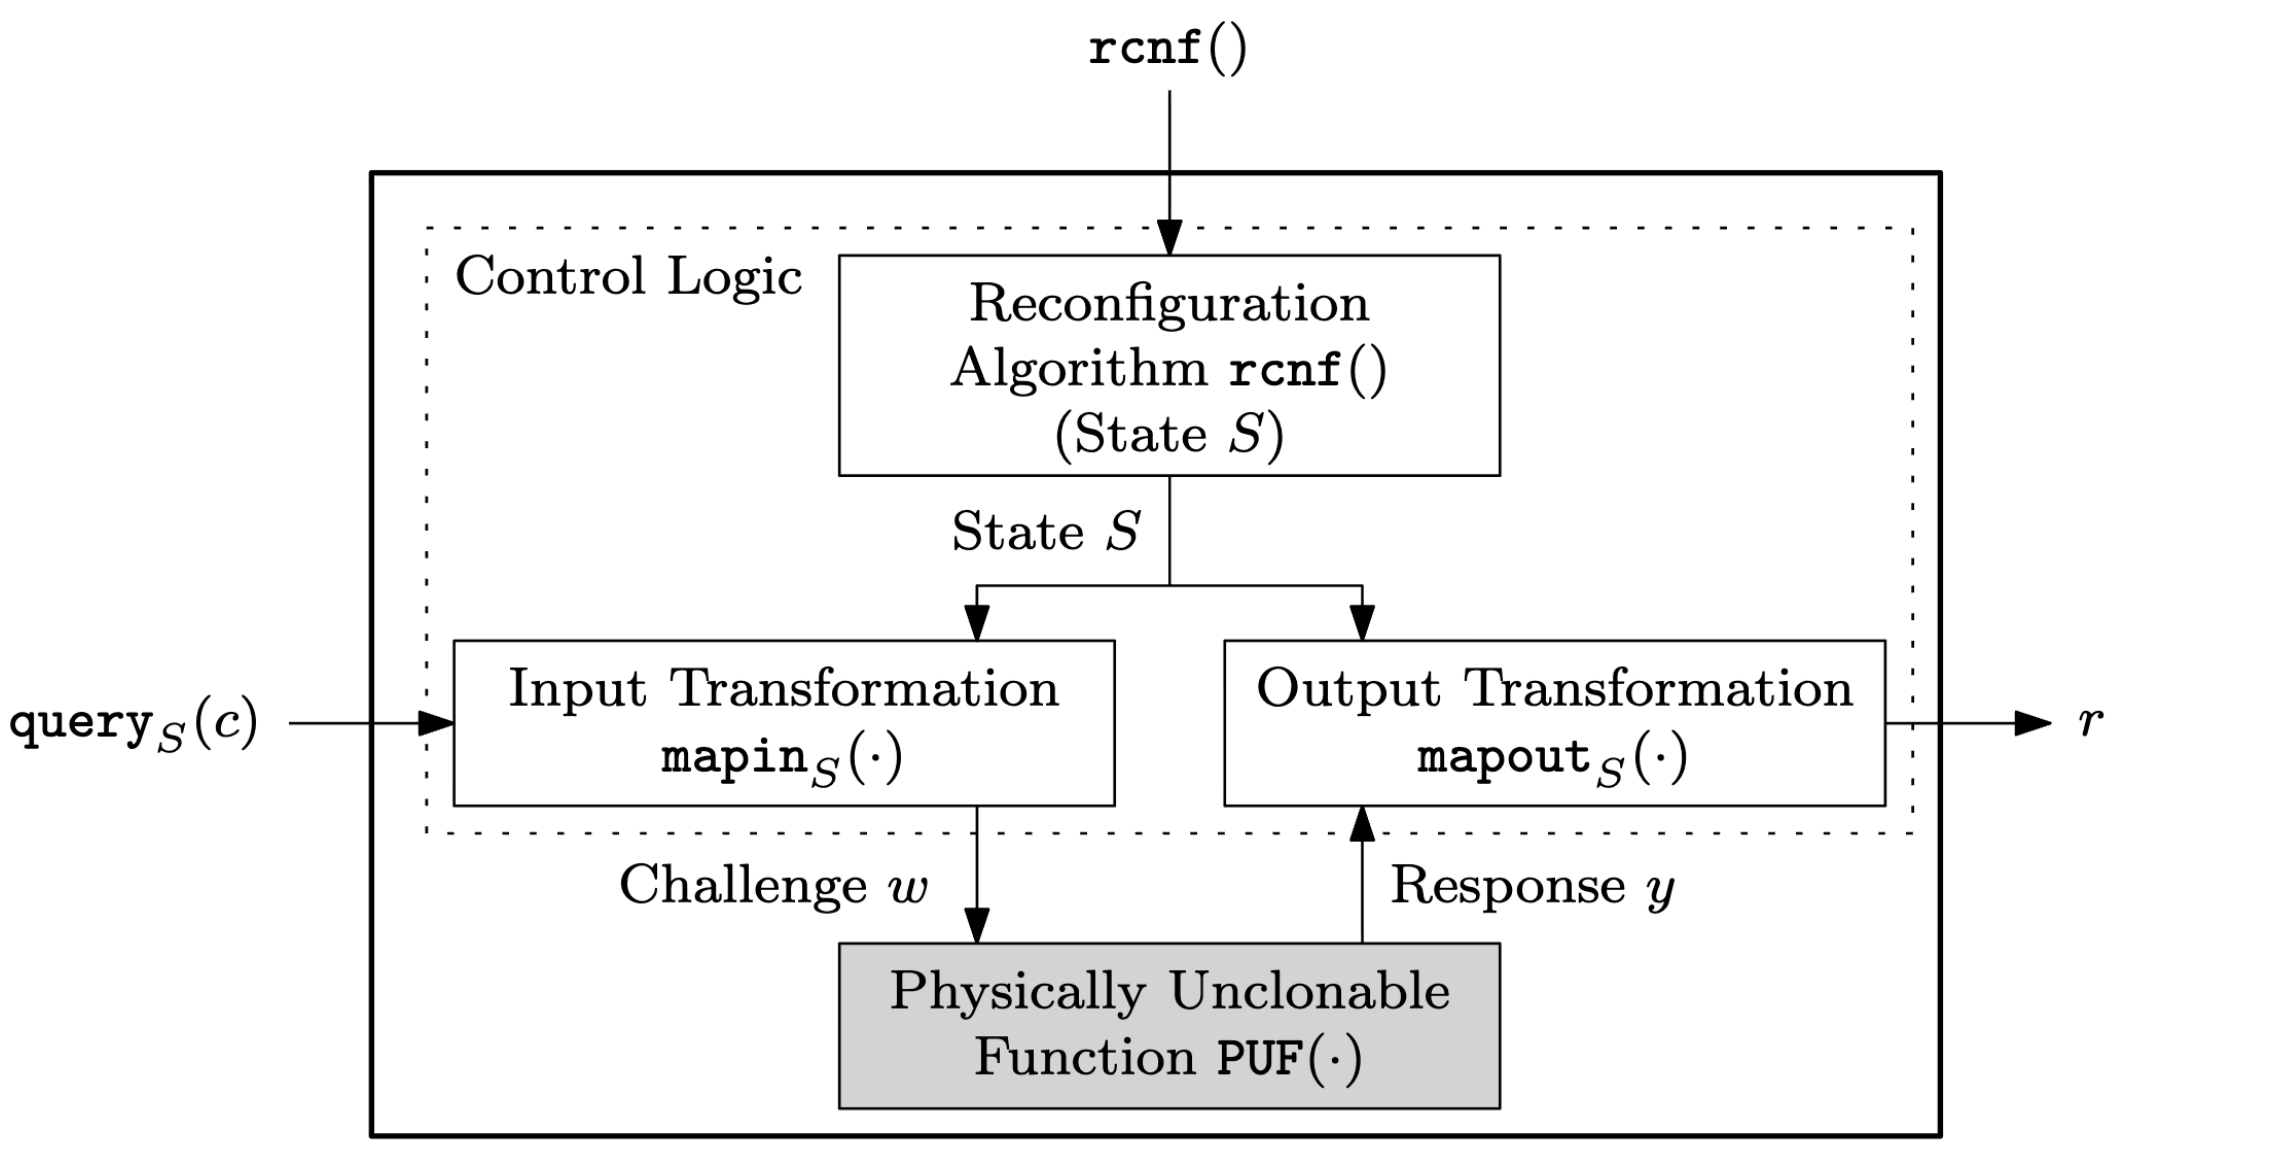
\includegraphics[width=1\linewidth]{img/LR-PUF-Paper-Fig.png}
    \caption{Logically Reconfigurable PUF Architecture \cite{10.1007/978-3-642-23951-9_25}}
    \label{fig:LR-PUF-Paper}
\end{figure}

The function $\texttt{query}_S(c)$ is described in algorithm \ref{alg:LRPUF-query-Paper}. First some challenge $c$ is mapped to another challenge $w$ using the state $S$, then $w$ is used to query the underlying PUF to obtain a response $y$, and finally the response $y$ is mapped out using the state $S$ to get a response $r$. In practice, $\texttt{mapin}_S(c)$ and $\texttt{mapout}_S(y)$ use hash functions to perform the mappings and entangle the state $S$ with the challenge $c$ and response $r$ so that changing $S$ via $\texttt{reconf}()$ (Algorithm \ref{alg:LRPUF-rcnf-Paper}) consequently alters the mapping and along with it the challenge-response behavior.

\begin{algorithm}[ht!]
\caption{$\texttt{query}_S(c)$}
\begin{algorithmic}[1]
    \Require Challenge $c$, current state $S$
    \Ensure Response $r$
    \State $w \leftarrow \texttt{mapin}_S(c)$ 
    \State $y \leftarrow PUF(w)$ 
    \State $r \leftarrow \texttt{mapout}_S(y)$ 
    \State \Return $r$
\end{algorithmic}
\label{alg:LRPUF-query-Paper}
\end{algorithm}

\begin{algorithm}[ht!]
\caption{$\texttt{rcnf}()$}
\begin{algorithmic}[1]
    \Require Current state $S$
    \Ensure New state $S'$
    \State $S' \leftarrow Hash(S)$
    \State $S \leftarrow S'$
\end{algorithmic}
\label{alg:LRPUF-rcnf-Paper}
\end{algorithm}

\newcommand{\Adv}{\mathcal{A}}

\subsection{Threat Model}
The underlying PUF of the LR-PUF is assumed to be physically unclonable and unpredictable. The algorithms for $\texttt{mapin}_S(c)$, $\texttt{mapout}_S(y)$ and $\texttt{reconf}()$ are assumed to be publicly known so as not to rely on security by obscurity. The adversary $\Adv$ is assumed to know the current state $S$ and all previous states of the LR-PUF, but $\Adv$ cannot alter $S$. Based on this threat model, the paper outlined the following properties of an LR-PUF:
\begin{itemize}
    \item \textbf{Backward unpredictability}: $\Adv$ cannot predict the response of the LR-PUF for a previous state to a challenge that has not been queried using that previous state, even if $\Adv$ knows a set of CRPs related to the previous state and can actively query the current state. In other words, once the LR-PUF has been reconfigured, an adversary who only interacts with the reconfigured LR-PUF cannot recover CRPs pertaining to the previous state. 
    \item \textbf{Forward unpredictability}: $\Adv$ cannot predict the response for the current state to a challenge that has not been queried using the current state, even if $\Adv$ knows a set of CRPs related to the previous state and can actively query the current state. In other words, an adversary who has fully compromised the LR-PUF before reconfiguration gains no advantage in predicting its behavior after reconfiguration.
    \item \textbf{Non-resettability}: $\Adv$ cannot set the state of the LR-PUF to a specific value, since this would allow $\Adv$ to trivially break backward unpredictability by resetting the state to a know compromised previous state.
\end{itemize}

The paper argues that non-resettability can be achieved in practice since arbitrarily modifying the state $S$ stored in non-volatile memory through an attack would be uneconomical given the needed precision and equipment.

\subsection{LR-PUF Construction Types}
The paper proposed two implementations of the LR-PUF. The first is optimized for speed and the second is optimized for space.

\subsubsection{Speed-Optimized Construction}
The speed-optimized construction uses a PUF with a large challenge-response space, i.e. a strong PUF. The CRP space must be large for this construction since otherwise it may be possible to enumerate all CRPs. The construction is described in algorithm \ref{alg:LRPUF-speed-query}. When querying, a challenge $w$ is computed by hashing the state $S$ along with the input challenge $c$, then $w$ is used to query the PUF and obtain $y$ which is given as the response $r$ of the LR-PUF. To reconfigure, the state is hashed into itself $S\leftarrow Hash(S)$. Speed here comes from the fact that the hash function is only called once and the PUF is also only queried once. 

\begin{algorithm}[ht!]
\caption{Speed-Optimized $\texttt{query}_S(c)$}
\begin{algorithmic}[1]
    \Require Challenge $c$, current state $S$
    \Ensure Response $r$
    \State $w \leftarrow Hash(S || c)$ \Comment{$\texttt{mapin}_S(c)$}
    \State $y \leftarrow PUF(w)$
    \State $r \leftarrow y$ \Comment{$\texttt{mapout}_S(y)$}
    \State \Return $r$
\end{algorithmic}
\label{alg:LRPUF-speed-query}
\end{algorithm}

\subsubsection{Area-Optimized}
Most PUF architectures with a large challenge space have a small response space, for example the Arbiter PUF. To get more response bits, more PUF cells are needed, but this significantly increases the needed physical area for the PUF. The area-optimized construction queries the PUF $n$ times to allow for more response bits. As described in algorithm \ref{alg:LRPUF-area-query}, a for loop queries the PUF $n$ times by deriving $n$ challenges $w_j \leftarrow Hash(S||c||j)$ and then finally combining their responses $y_j$ into $r \leftarrow (y_0 || \dots || y_n)$.


\begin{algorithm}[ht!]
\caption{Area-Optimized $\texttt{query}_S(c)$}
\begin{algorithmic}[1]
    \Require Challenge $c$, current state $S$, number of sequential PUF evaluations $n$
    \Ensure Response $r$
    \For{$j = 0$ to $n$}
        \State $w_j \leftarrow Hash(S || c || j)$ \Comment{$\texttt{mapin}_S(c)$}
        \State $y_j \leftarrow PUF(w_j)$
    \EndFor
    \State $r \leftarrow (y_0 || \dots || y_n)$ \Comment{$\texttt{mapout}_S(y)$}
    \State \Return $r$
\end{algorithmic}
\label{alg:LRPUF-area-query}
\end{algorithm} 

\subsection{Performance Evaluation}
Both constructions were implemented on a Xilinx Spartan-6 FPGA board. The underlying PUF is an Arbiter PUF with 64-bit challenges and 1-bit responses. Both resulting constructions take 80-bit challenges and generate 64-bit responses. Table \ref{tab:lrpuf-perf-paper} shows their results.

\begin{table}[ht!]
\centering
\caption{Performance results of the speed- and area-optimized LR-PUF constructions \cite{10.1007/978-3-642-23951-9_25}.}
\begin{tabular}{lccc}
\hline
\textbf{Construction} & \textbf{Response time} & \multicolumn{2}{c}{\textbf{Area consumption in slices}} \\
 & \textbf{(clock cycles)} & \textbf{Control logic} & \textbf{Arbiter PUF} \\
\hline
Speed-optimized & 1,069    & 166 & 4,288 \\
Area-optimized  & 64,165   & 358 & 67    \\
\hline
\end{tabular}
\label{tab:lrpuf-perf-paper}
\end{table}

The area-optimized construction requires only about 27\% of the total area required for the speed-optimized construction, but it is about 60 times slower for producing a response. Note that the implementation did not account for the non-volatile memory required to store the state $S$.

\section{Field Programmable Gate Array (FPGA)}
A Field Programmable Gate Array (FPGA) is an integrated circuit whose internal digital logic is not fixed at manufacturing time but can instead be reconfigured to implement almost any digital circuit. It stands in direct contrast to Application-Specific Integrated Circuits (ASIC), whose logic is permanently set during fabrication, and to micro-controller units (MCU), whose fixed hardware can execute sequential instructions. FPGAs stand in the middle between ASIC and MCU. 

\subsection{Architecture}
According to \cite{2018arXiv180503648K}, an FPGA is built from a few recurring building blocks (Figure \ref{fig:fpga-architecture}):
\begin{itemize}
    \item \textbf{Slices}: A slice is a small cluster of look-up tables (LUT) and flip-flops (FF) repeated thousands of times across the FPGA chip. A LUT can be programmed to compute any boolean function of its inputs by writing the function's truth table into it, and an FF is used to store the LUT's output on the next clock edge to build sequential logic. 
    \item \textbf{Programmable Interconnect}: Slices are connected to one another through routing channels and switch-boxes, which are configurable switches that wire one signal path to another.
    \item \textbf{Hardened Blocks}: Some operations are needed so often that building them out of slices would be wasteful. FPGAs therefore embed purpose-specific non-reconfigurable blocks for such operations. The most common are Block RAM (BRAM) for on-chip storage, dedicated micro-processors for running custom firmware, and dedicated DSP (Digital Signal Processing) blocks for optimizing mathematical operations.
\end{itemize}

\begin{figure}
    \centering
    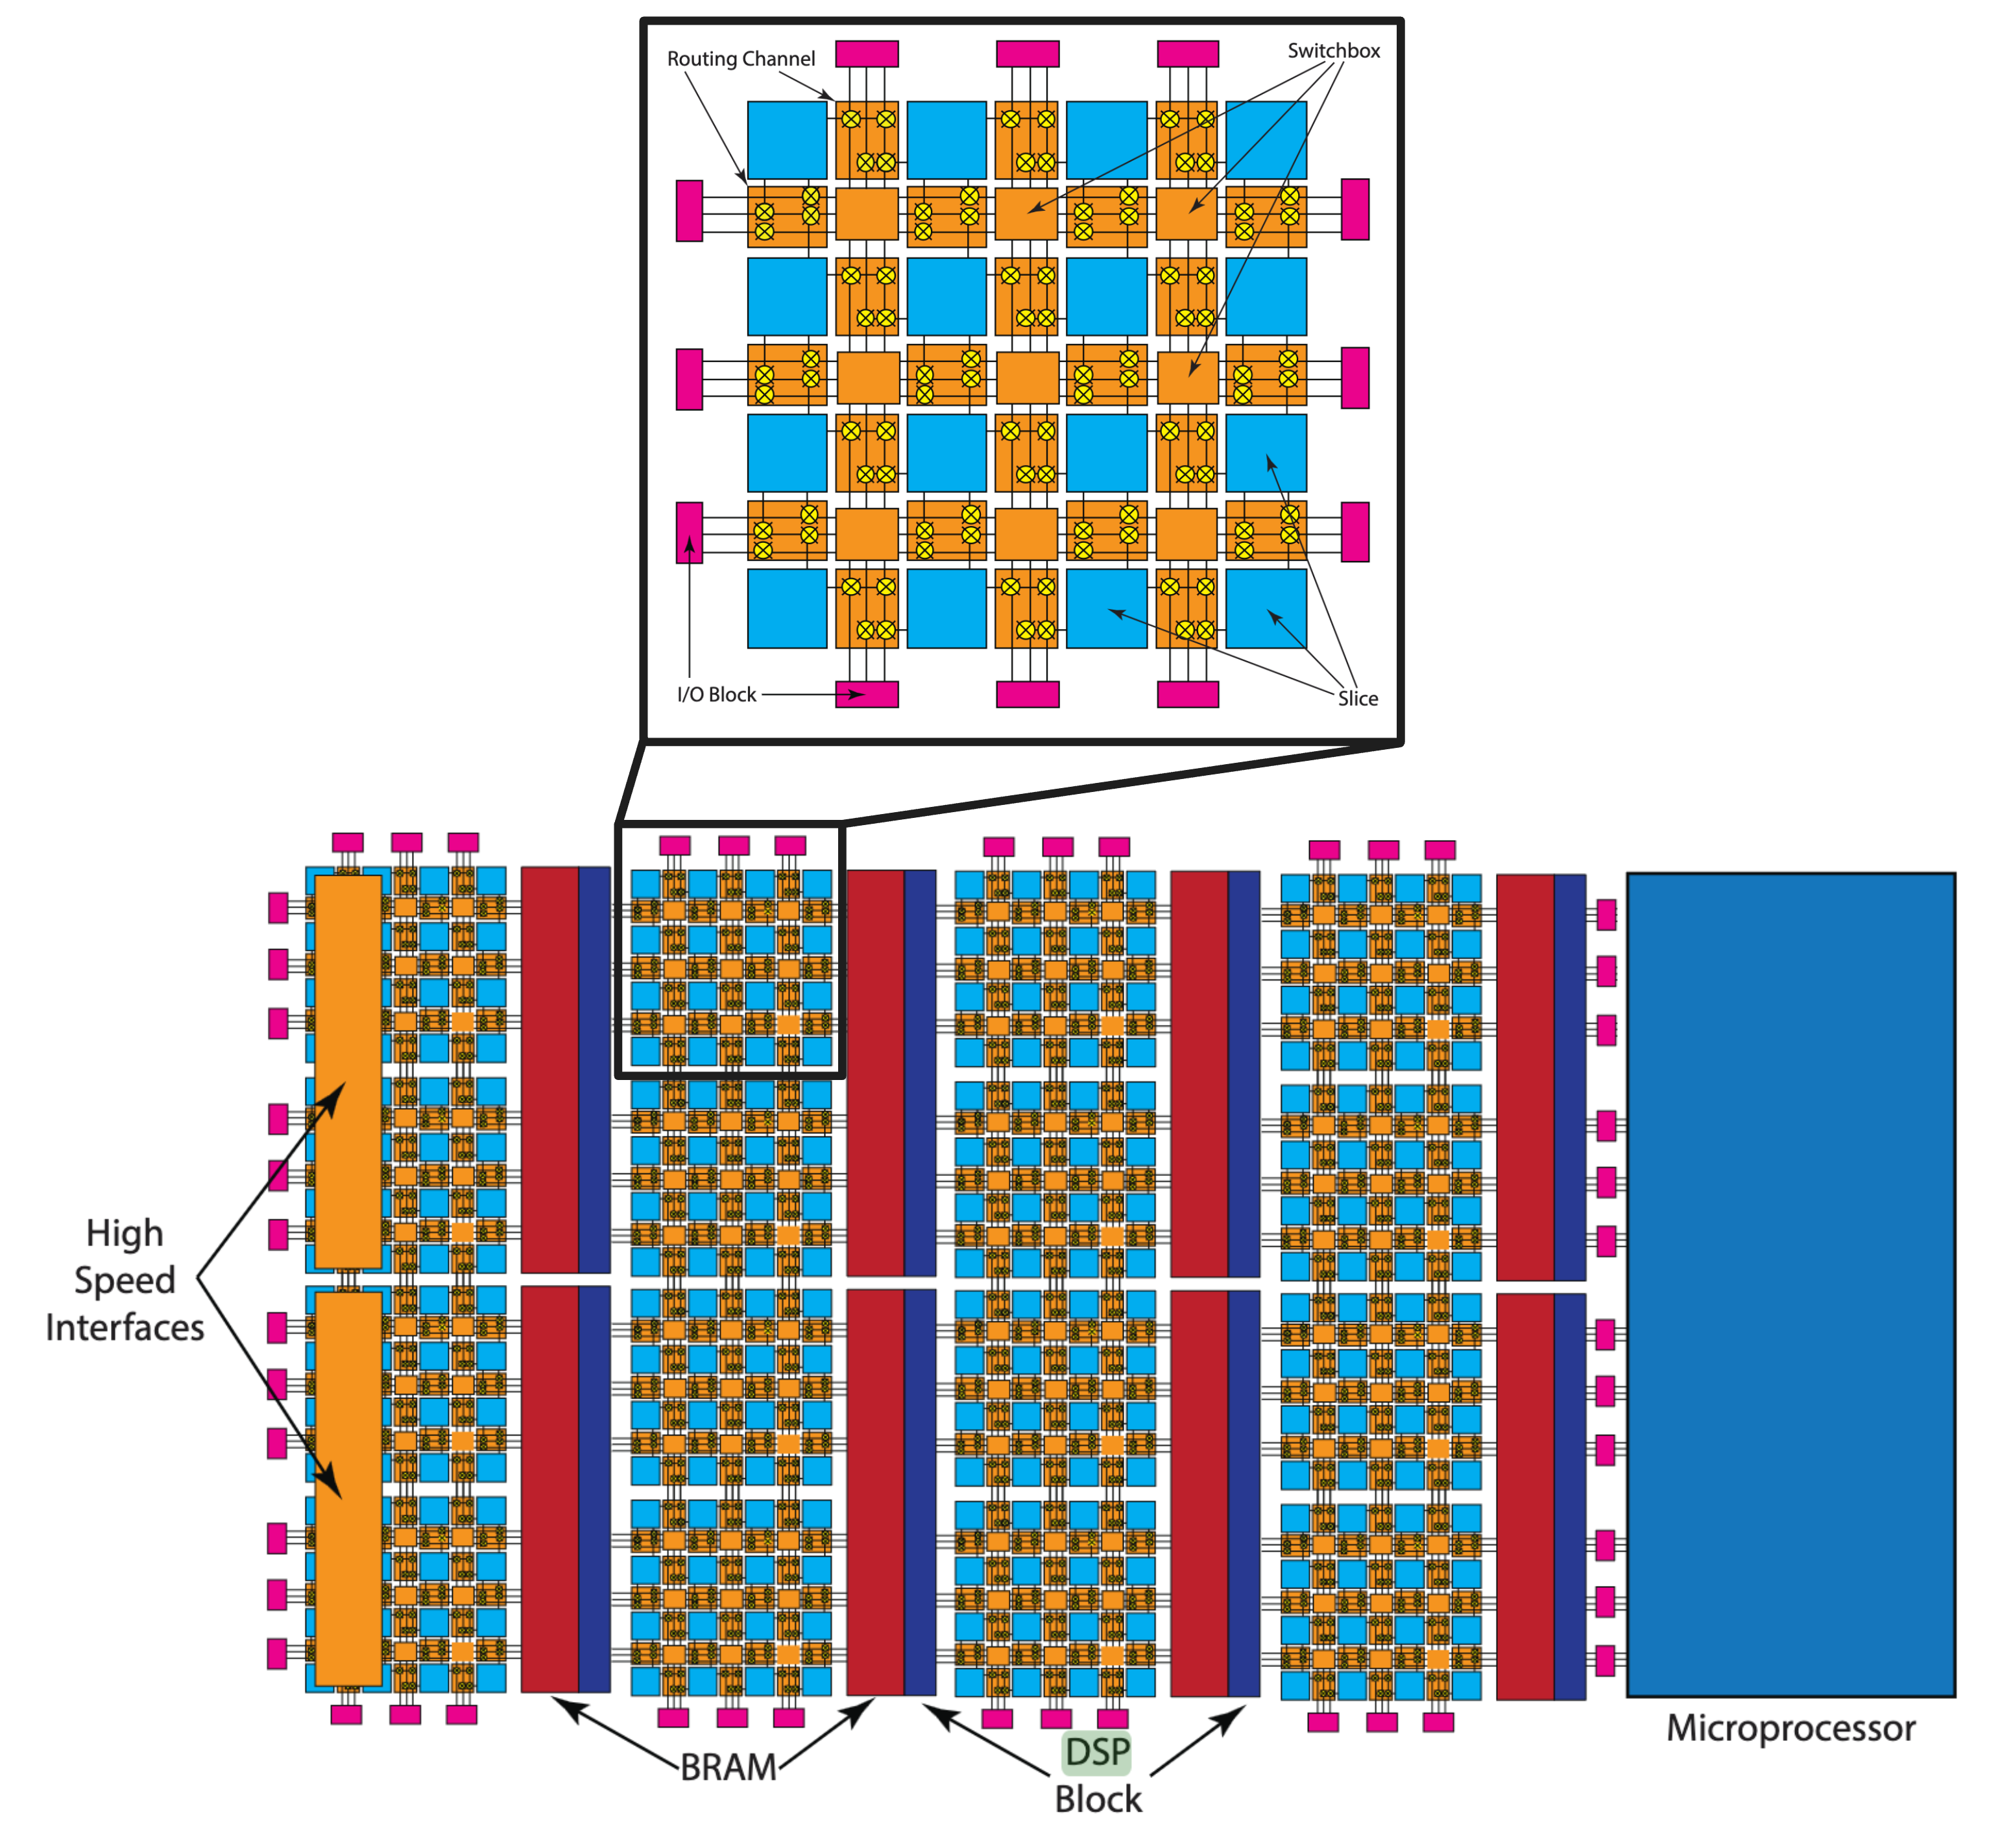
\includegraphics[width=1\linewidth]{img/FPGA-Diagram.png}
    \caption{FPGA Architecture \cite{2018arXiv180503648K}}
    \label{fig:fpga-architecture}
\end{figure}

\subsection{Design Pipeline}
To program a circuit into an FPGA, it must be described using a Hardware Description Language (HDL) such as Verilog or VHDL. The HDL code is elaborated into a Register Transfer Level (RTL) netlist, which is a technology-independent representation that describes the circuit in terms of registers and logic operations. This RTL representation is then synthesized into a netlist of basic logic gates, which are then placed and routed onto the FPGA's actual slices and programmable interconnects, and finally packaged into a bitstream, which is a binary file that configures every LUT, FF and switch on the chip.

\section{Session Hijacking}
Web applications are built on top of the HTTP protocol. HTTP is stateless, which means that by default the server treats every incoming request independently and retains no memory of any previous request from the same client. To identify and authenticate a user across multiple requests, a session is created and used. A session is a period of authenticated interaction that begins once the user successfully logs in and lasts until the user ends it or if it reaches its expiry. Once a session is established, the server issues a session token, which is typically stored in a cookie \cite{rfc6265} to uniquely identify the session. The browser presents this cookie to every subsequent request sent to the server, and the server considers any request carrying a valid token as coming from an authenticated user.

Session Hijacking is an attack in which an adversary obtains a victim's session token and uses it to act as the victim to the server. Because the server authenticates a request purely based on possession of a valid token, a request carrying a stolen token is indistinguishable from a legitimate request. Once the token is in the attacker's possession, they gain full access to the victim's account for as long as the token remains valid without needing to know the victim's credentials. This means that Session Hijacking bypasses Multi-Factor Authentication (MFA), since MFA only protects the initial login step, but once a token is issued, the token alone is sufficient to keep using the session with no further proof of identity required until it expires. This motivates session hijacking countering approaches using Continuous Authentication (CA), where a session is continuously verified during use, so that even a stolen token is not by itself sufficient to keep a session alive.

A session token can be stolen through different means:
\begin{itemize}
    \item \textbf{Malware}: The most common vector is through dedicated cookie-stealing malware, also known as "Infostealer". The victim is tricked into running the malware on their own machine through social engineering \cite{shen2021phishing}.
    \item \textbf{Cross-Site Scripting (XSS)}: If an XSS vulnerability exists in the web app, an attacker can get malicious JavaScript to execute in the victim's browser and exfiltrate the session token stored in the cookies. However, this attack vector is mostly outdated since the new \verb|HttpOnly| flag on cookies makes them inaccessible from JavaScript, but exceptions could exist where some web apps still do not use \verb|HttpOnly| on sensitive cookies. 
    \item \textbf{Network Interception}: An attacker positioned between the victim and the server, for example through an adversary-in-the-middle phishing proxy \cite{evilginx2_kgretzky_2024}, can relay the victim's traffic to the real server and capture the session token as it passes through.
\end{itemize}

\section{PUSH Protocol}
PUSH (PUF against Session Hijacking) \cite{10.1007/978-3-032-07894-0_7} is a protocol that mitigates session hijacking. It works by binding the session to a physical USB dongle whose identity is derived from a PUF, and by periodically requiring that dongle to re-prove its presence for as long as the session remains active. It is the first protocol to apply PUF-based hardware binding to session hijacking for web security. The proposed REPUSH protocol in this thesis builds directly on PUSH.

\subsection{System Model}
PUSH involves four parties (Figure \ref{fig:push-parties}):
\begin{itemize}
    \item \textbf{The dongle}: an external USB device containing an SRAM PUF module and a crypto module. The crypto module is responsible for querying the PUF and deriving cryptographic keys from it to produce digital signatures.
    \item \textbf{PUFMAN (PUF Manager)}: a background service running on the user's device that communicates to the dongle over USB and exposes an API to the browser to allow it to use the dongle.
    \item \textbf{The browser}: acts as the client through which the user communicates with the server or web application.
    \item \textbf{The server}: the web application or service.
\end{itemize}
The dongle, the user's device, PUFMAN and the server are all assumed to be trusted, but the browser is treated as potentially exposed to malicious extensions. PUSH operates at the application layer on top of HTTPS, and assumes that session cookies are handled and stored securely using the standard mechanisms.

\begin{figure}
    \centering
    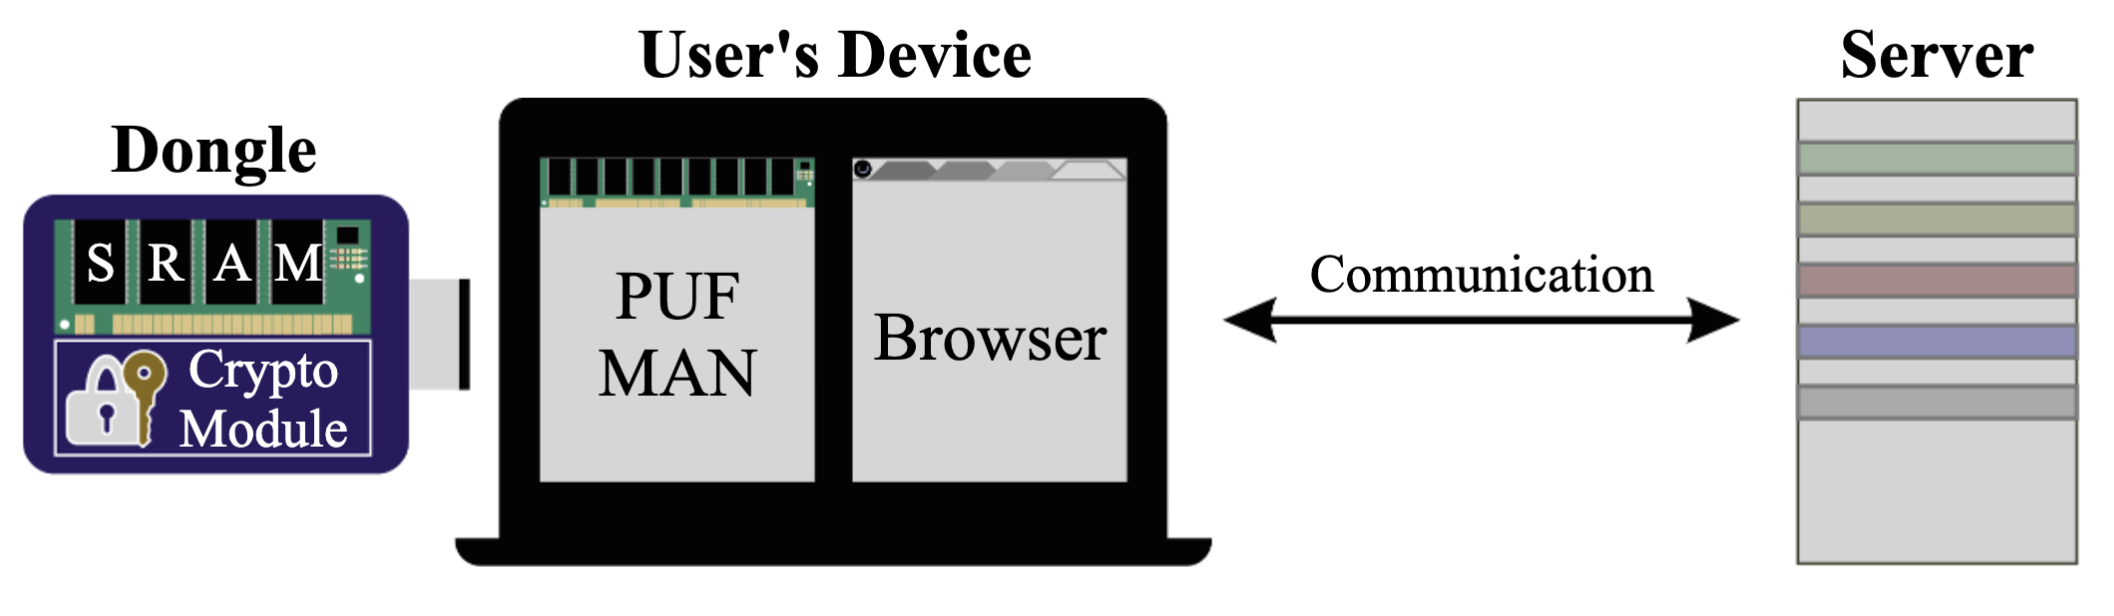
\includegraphics[width=1\linewidth]{img/PUSH-parties.png}
    \caption{PUSH parties. \cite{10.1007/978-3-032-07894-0_7}}
    \label{fig:push-parties}
\end{figure}

\subsection{Protocol Phases}
PUSH is composed of three phases: a one-time dongle initialization, a one-time enrollment with the server, and a recurring operation phase.

\subsubsection{Phase 1: PUF Initialization}
The objective of this phase (Figure \ref{fig:push-init}) is to derive a stable fingerprint from the dongle's SRAM PUF and turn it into a key pair. The crypto module power-cycles the SRAM module $k$ times and reads its contents, which are in this case the SRAM PUF responses. Then the average hamming distance and hamming weight for each memory cell is computed to determine reliable and uniform cells. This filtered set of addresses forms the PUF challenge $C$, and their corresponding bit values form the response $R$. $CRP = (C,R)$ then acts as the unique fingerprint of the dongle. $R$ is processed using a fuzzy extractor to later error-correct it, and the result is used to seed a key generation function $KeyGen()$ for producing a  key pair $(SK, PK)$. Finally, the crypto module signs both $C$ and $PK$ using a secret manufacturer-issued key $SK_D$, and sends $C$, $PK$, and the two signatures to PUFMAN. Once this phase completes, the SRAM module is powered off and both $SK$ and $PK$ are discarded. From now on, the key pair is reconstructed on-demand directly from the PUF rather than being stored on memory.
\begin{figure}
    \centering
    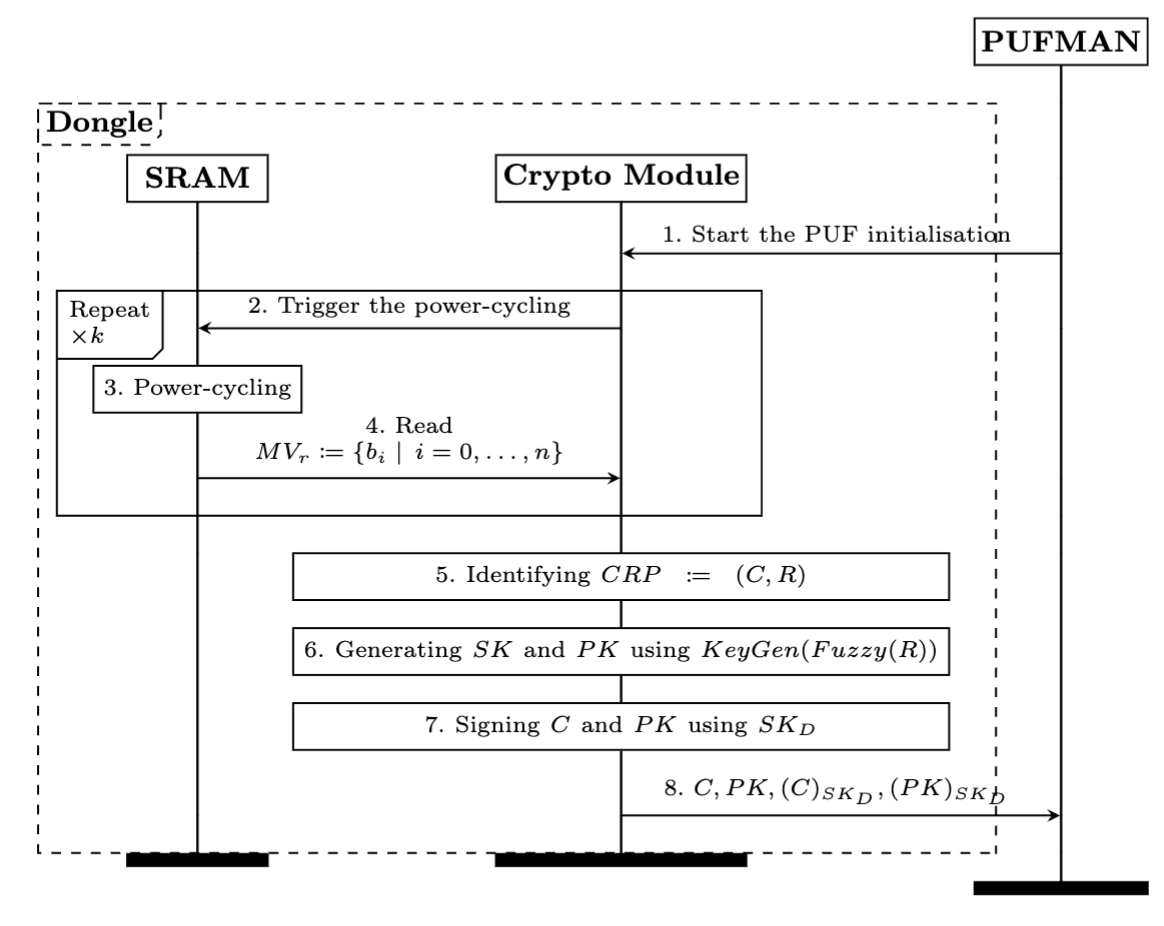
\includegraphics[width=0.7\linewidth]{img/PUSH-init.png}
    \caption{PUSH initialization phase \cite{10.1007/978-3-032-07894-0_7}}
    \label{fig:push-init}
\end{figure}

\subsection{Phase 2: Enrollment}
The user provides the browser with the dongle's manufacturer-issued public key $PK_D$, which the browser uses to validate the produced signatures on $C$ and $PK$ obtained via PUFMAN. The browser does this to confirm that the dongle is genuine. Once validated, the browser sends $C$ and $PK$ to the server as an enrollment request. The server creates a new session for the user, assigns it a session ID, and returns it to the browser as a cookie. From now on, the session is established.
\begin{figure}
    \centering
    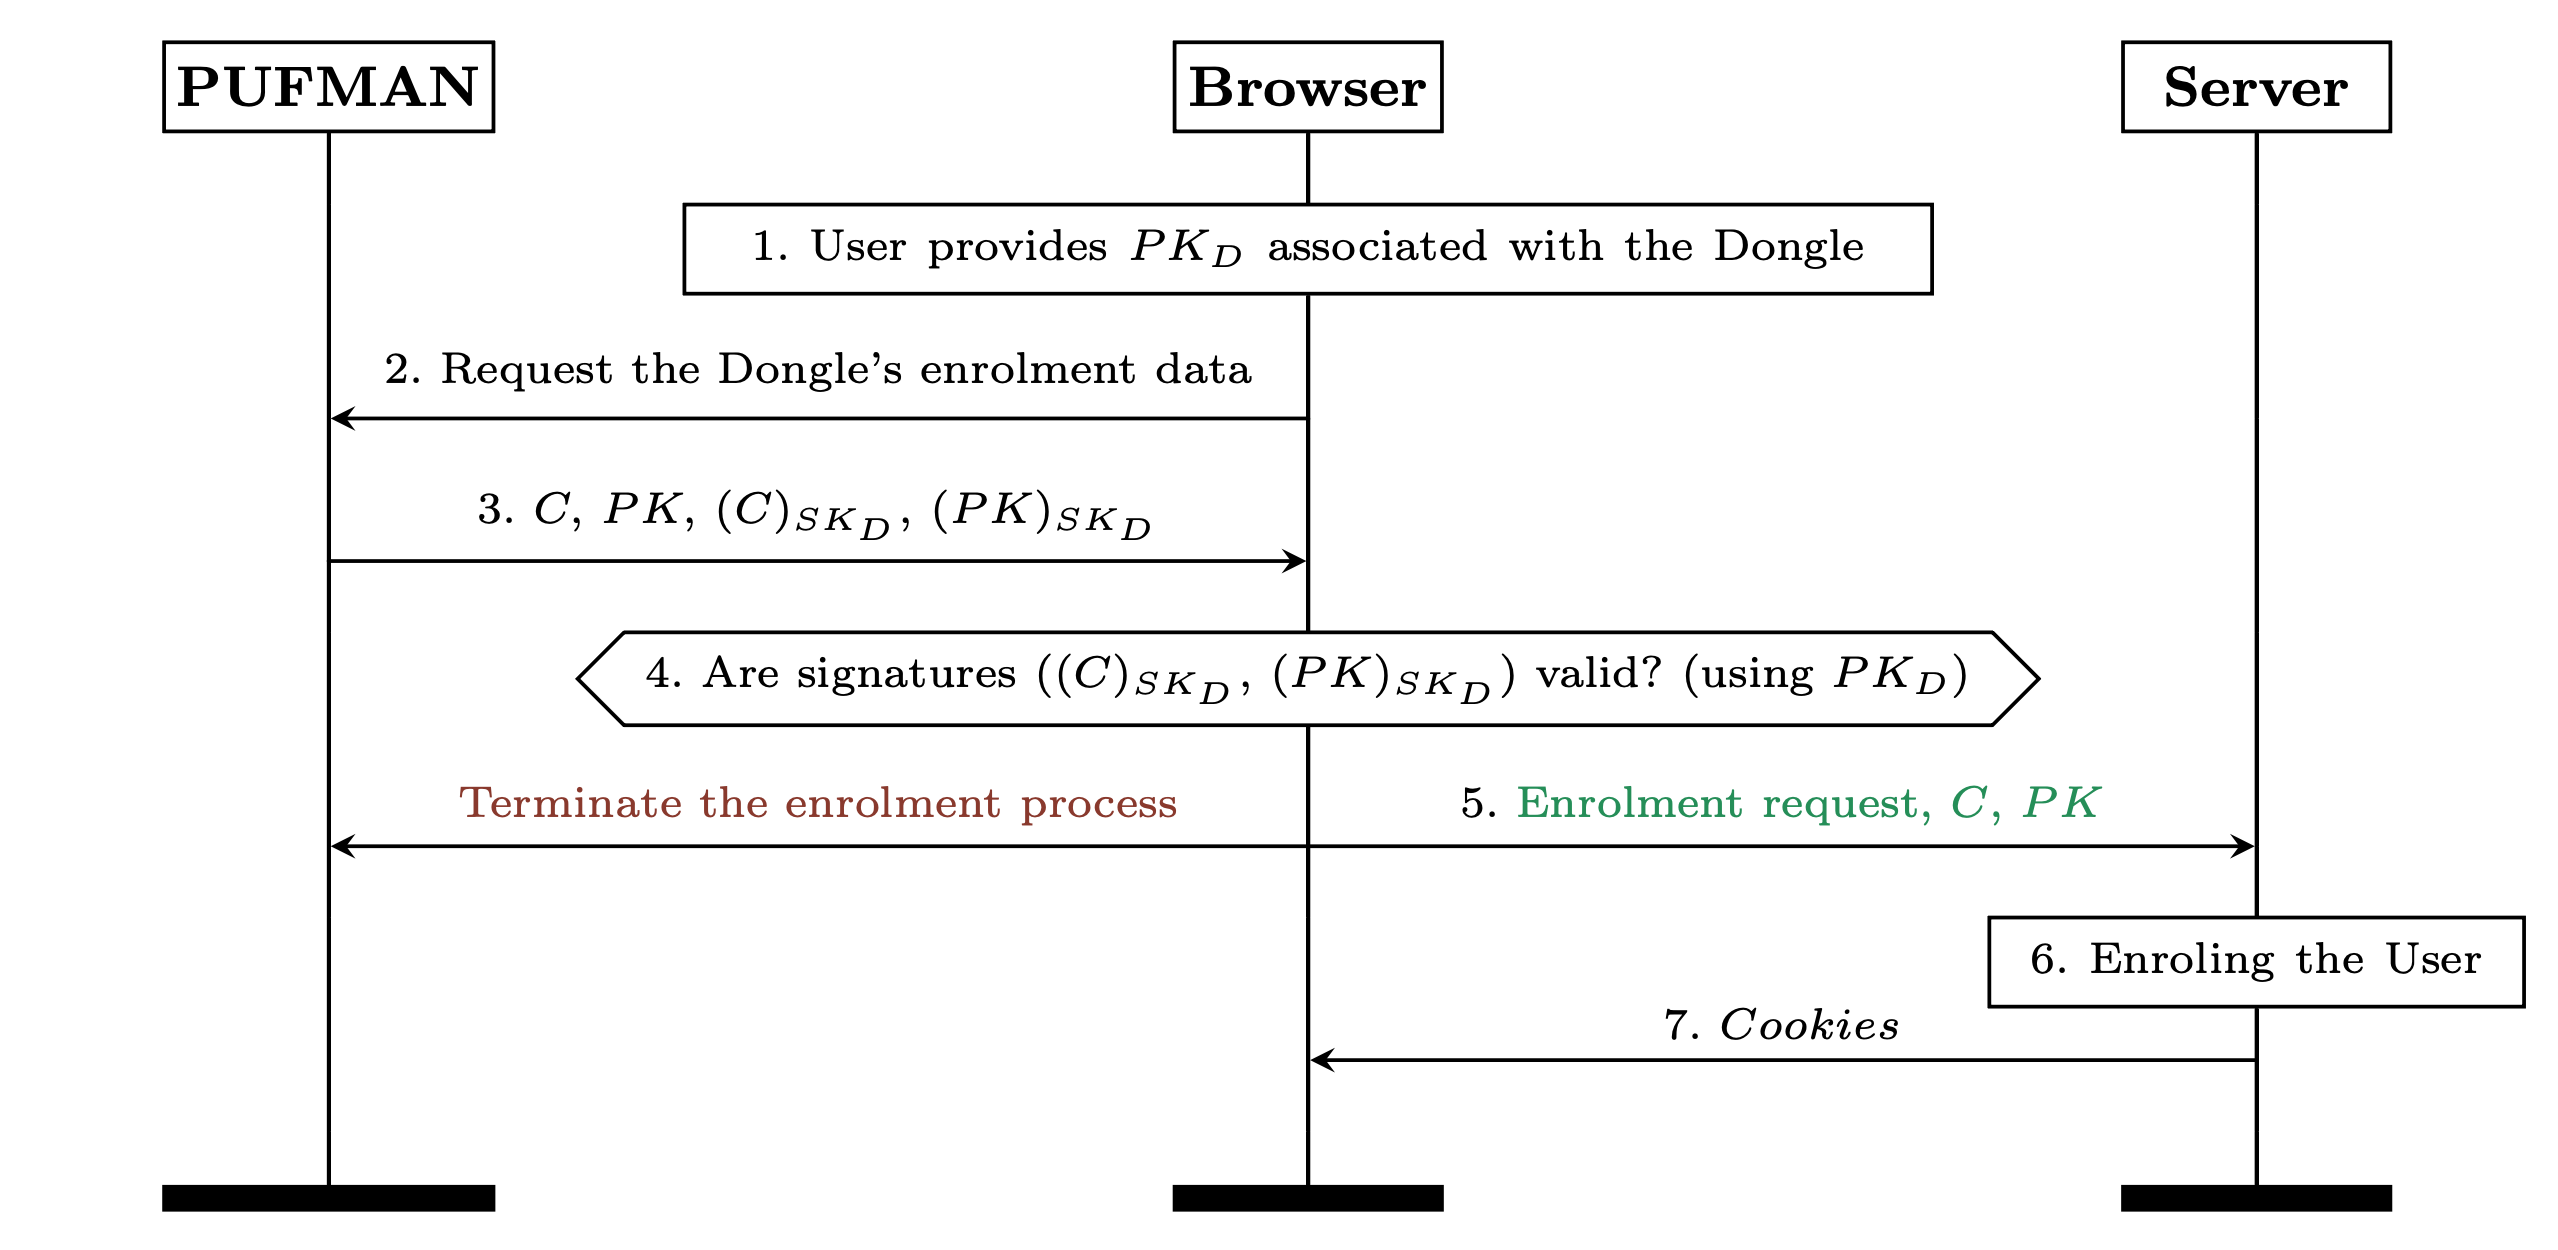
\includegraphics[width=0.7\linewidth]{img/PUSH-enroll.png}
    \caption{PUSH enrollment phase \cite{10.1007/978-3-032-07894-0_7}}
    \label{fig:push-enroll}
\end{figure}

\subsection{Phase 3: Operation}
For every subsequent request, the browser attaches the cookie to it as usual. However, the server periodically responds by also including the enrolled challenge $C$ together with a freshly generated nonce $N$ to be signed along with the cookie by the dongle. This request is relayed to the dongle via the browser and PUFMAN. The dongle queries the SRAM PUF by powering on the SRAM and reading the response $R$ using the addresses specified by $C$. Since this new reading $R$ is subject to noise, it must be error-corrected using the fuzzy extractor before using it to regenerate the key pair $(SK,PK)$ derived in phase 1. $SK$ is then used to sign $N$ and the cookie. The resulting signatures are relayed back to the server, which will either accept them if the nonce $N$ is fresh and both signatures are correct under $PK$, otherwise, the session is terminated. Requesting a signature on every single request would introduce noticeable latency, so instead the signature is treated as valid for a specific validity window and is refreshed shortly before it expires at some update time $T_{update} < T_{validity}$. A shorter $T_{validity}$ terminates a hijacked session more quickly, but requires more frequent signing.
\begin{figure}
    \centering
    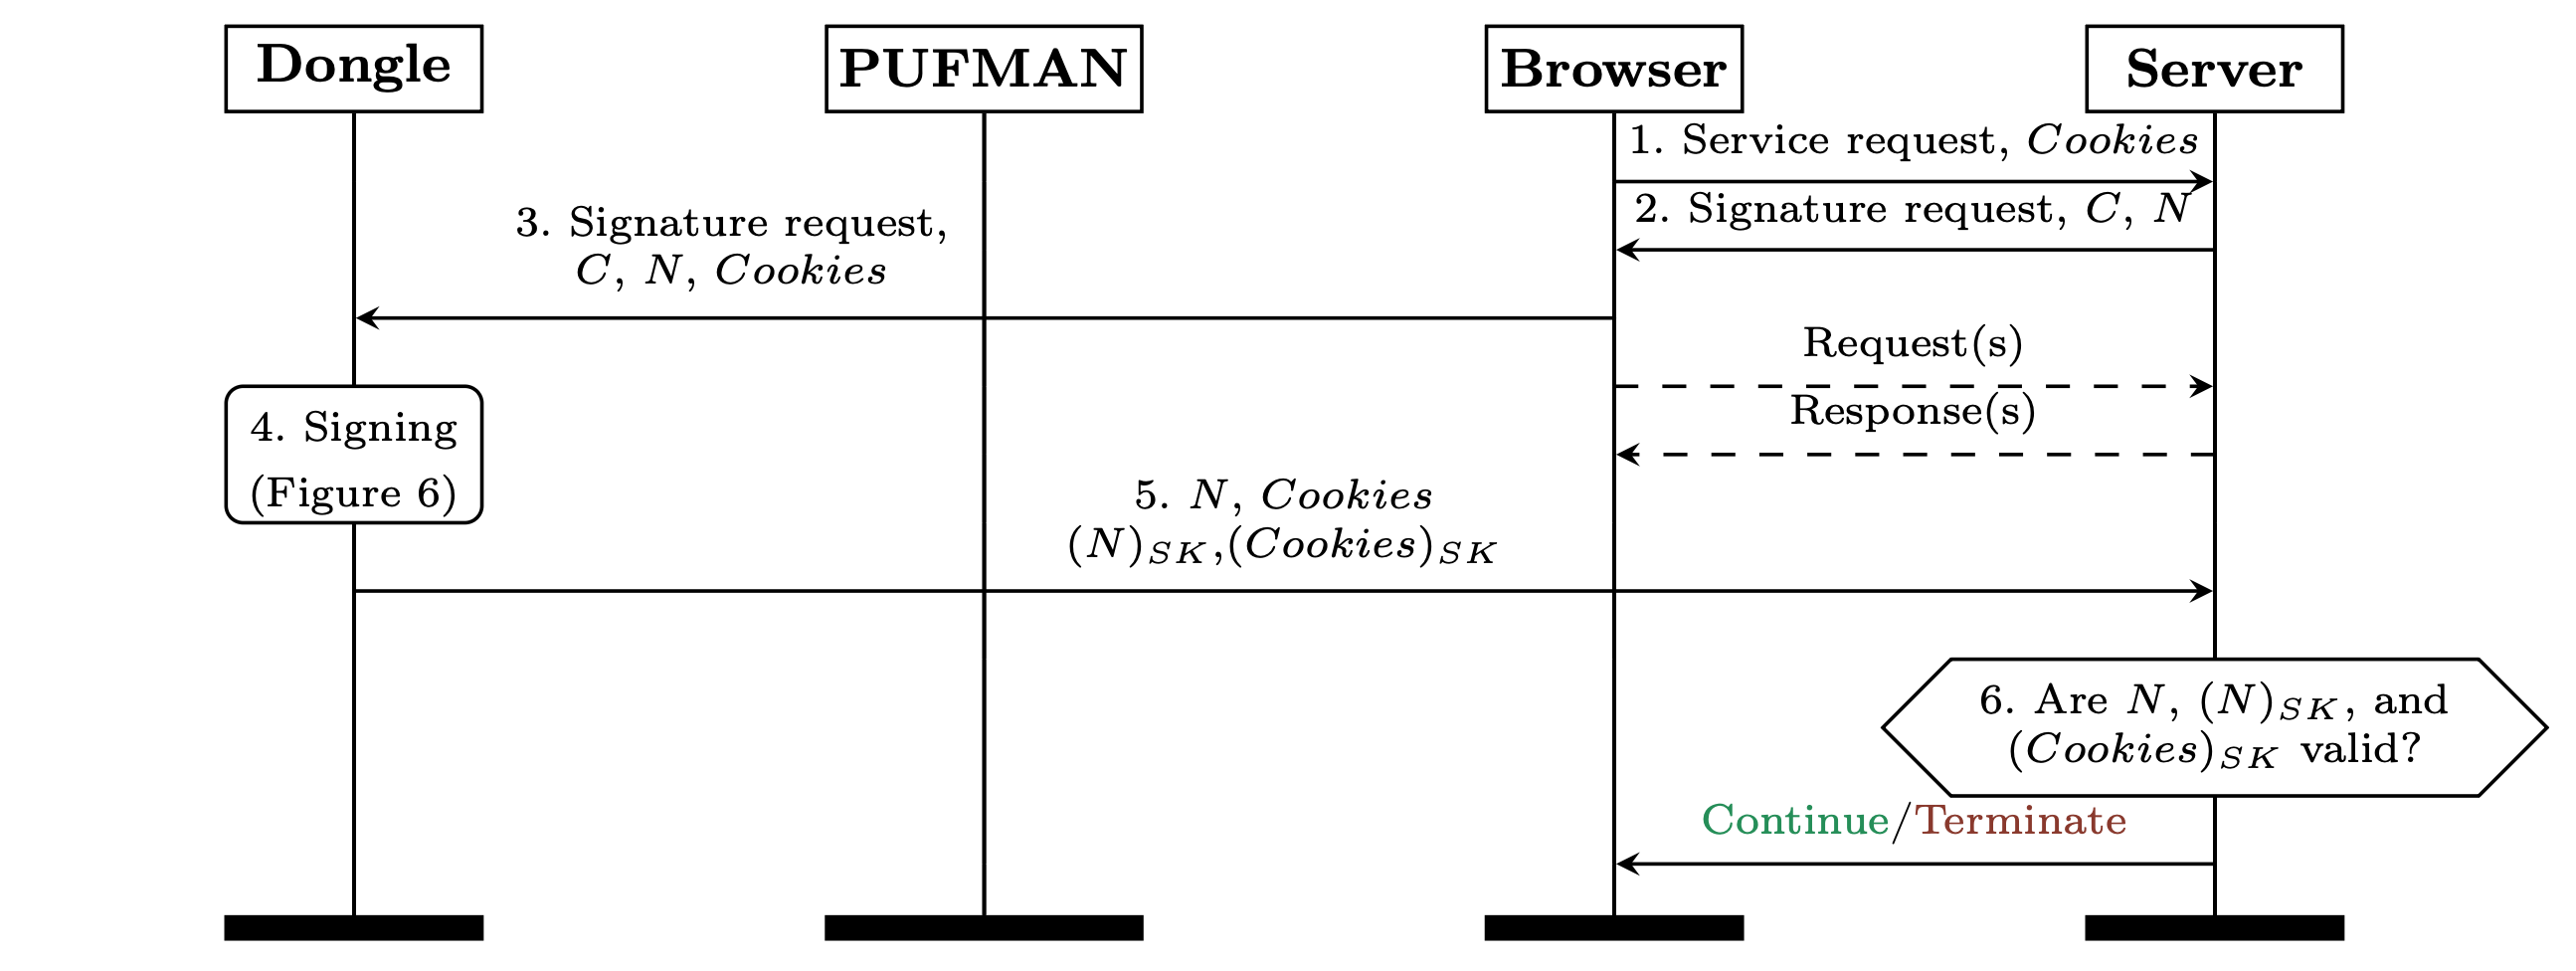
\includegraphics[width=0.9\linewidth]{img/PUSH-oper.png}
    \caption{PUSH operation phase \cite{10.1007/978-3-032-07894-0_7}}
    \label{fig:push-oper}
\end{figure}

\subsection{Performance and Limitations}
In PUSH's proof-of-concept implementation, the dongle is built using an Arduino Nano 33 BLE board with an external SRAM module and Curve25519 signing. Phase 1 for PUF initialization took around 11 seconds, which is dominated by the time need to power-cycle the SRAM three times ($k=3$). Phase 2 for enrollment took around 2 ms. The signing during the operation phase took in average 419 ms. Since initialization only runs once and the signatures only happen periodically, PUSH introduces very little latency in practice.

PUSH has some limitations. For example, PUSH's scalability is bounded by the size of the SRAM PUF. Since each session requires its own unique CRP, the total number of concurrent sessions the dongle can support is limited by how many disjoint CRPs can be extracted from the SRAM. The other limitations were discussed as part of the introduction to this thesis.

